% Author: Carles Marin (Claude, Anthropic, as AI research assistant).
% Part VI. One row of their table: proton stability in SU(7) grand gauge-Higgs unification.
% Komori-Maru (arXiv:2503.04090) leave proton decay to future work. Their own anomaly cancellation
% forces the leftover U(1)' to be T3L + Y - (B-L), a span every dimension-6 |dB|=1 operator is
% neutral under, and two channels that cannot cancel demand a right-handed neutrino of U(1)' charge
% -1, which lives in the 28 and nowhere else. The escape is a family-dependent charge, available as
% a ladder inside their own SU(7), hosted by an 84(+,+) that every row of their Table 1 already
% contains. Donating that 84 removes it from their Higgs potential by their own argument, at an
% exact cost D = 5/4. Case (3) has only 9/8, so case (2) is the only one of the five published rows
% that does both -- within the minimal extension, at one-loop curvature. A benchmark SELECTED, not a
% model delivered: the modified potential is not recomputed here.
% NOT claimed anywhere: a defect in their paper. Their Table 1 alpha_min is not reproduced from
% their published formulas; that is recorded as an open question, and section 7 shows the conclusion
% is invariant over the whole family of repairs that failure allows.
% English edition; the Spanish one is made once this text stops moving.
% Build: pdflatex x2.  Every displayed number regenerates from ../*.py and ../*.sage, output
% archived in ../outputs/; the figures are drawn by ../make_figures_su7.py from ../paper_data/.
\documentclass[11pt,a4paper]{article}
\usepackage{cmap}   % ToUnicode CMaps: ligatures and _ must survive copy/paste and full-text search
\usepackage[utf8]{inputenc}
\usepackage[T1]{fontenc}   % OT1 draws \_ as a RULE, not a glyph: script names would not copy out
\usepackage{amsmath,amssymb,amsthm}
\usepackage{booktabs}
\usepackage{longtable}
\usepackage[table,dvipsnames]{xcolor}
\usepackage{graphicx}
\usepackage{tikz}
\usetikzlibrary{arrows.meta,positioning,decorations.pathmorphing}
\usepackage{geometry}
\geometry{margin=2.4cm}
\definecolor{softgrey}{RGB}{244,243,240}
\usepackage[colorlinks=true,linkcolor=RoyalBlue,citecolor=BrickRed,urlcolor=RoyalBlue]{hyperref}
\usepackage{caption}
\captionsetup{font=small,labelfont=bf}
\newtheorem{theorem}{Theorem}
\newtheorem{lemma}{Lemma}
\newtheorem{proposition}{Proposition}
\newtheorem{observation}{Observation}
\newcommand{\ZZ}{\mathbb{Z}}
\newcommand{\su}[1]{SU(#1)}
\newcommand{\rep}[1]{\mathbf{#1}}
\newcommand{\amin}{\alpha_{\min}}
\definecolor{hdrblue}{RGB}{31,78,121}
\definecolor{warmred}{RGB}{178,34,34}
\definecolor{okgreen}{RGB}{0,140,54}
\definecolor{amber}{RGB}{176,120,20}

% the thread: each section ends with the question the next one answers
\newcommand{\bridge}[1]{\par\medskip\noindent
  \textcolor{hdrblue!45}{\rule{2.2cm}{0.6pt}}\;\;\parbox[t]{0.84\textwidth}{\small\itshape
  \textcolor{hdrblue!85}{#1}}\par\medskip}

% a framed display for the statements the paper stands on -- and only those
\newsavebox{\keyeqbox}
\newenvironment{keyeq}
  {\begin{center}\setlength{\fboxsep}{9pt}\setlength{\fboxrule}{0.8pt}%
   \begin{lrbox}{\keyeqbox}\begin{minipage}{0.88\textwidth}}
  {\end{minipage}\end{lrbox}%
   \fcolorbox{hdrblue!55}{hdrblue!6}{\usebox{\keyeqbox}}\end{center}}

\title{\textbf{\Large Proton decay in $\su7$ grand gauge-Higgs unification:}\\[2pt]
\textbf{\Large an obstruction, its minimal escapes, and the one row}\\[2pt]
\textbf{\Large of their Table~1 that can pay for them}\\[7pt]
\large\textnormal{\itshape Anomaly cancellation forces the model's leftover $U(1)'$ to be
$T_{3L}+Y-(B-L)$, which no dimension-6 baryon-number-violating operator can see, and demands a
right-handed neutrino that exists in exactly one of the representations used --- an obstruction to
the model \textnormal{as published}. The escapes are then classified inside its own group, two of
them survive, and spending either costs a rational number that only one row of the published table
can afford.}\\[8pt]
\normalsize\textnormal{Part VI --- a study of the proton-decay question Komori and Maru pose, and
explicitly leave open, in arXiv:2503.04090. It does not close it. Working entirely inside their
construction and with their own equations, it finds that the one-generation version cannot forbid
the dangerous operators, classifies the minimal extensions that can, and shows that their Table~1
already contains the multiplet every one of them needs --- with one row able to afford it. Over a
third of the length goes to checking our own instrument rather than theirs: three of their equations
are re-derived here instead of assumed, and all three come out right; what we cannot yet reproduce is
one column of their table, and that is recorded as a question of ours. One row-independent invariant
is offered along the way, against which any table of this kind can be checked, ours included}}
\author{Carles Mar\'in\thanks{Independent researcher, \texttt{karlesmarin@gmail.com}.
The computations were carried out and cross-checked with Claude (Anthropic) as an AI research
assistant against a common machine-verifiable ground truth; every number in this paper regenerates
from the ancillary scripts, whose output is archived beside them.}}
\date{\today}

\begin{document}
\maketitle

\begin{abstract}
\noindent
Komori and Maru's $\su7$ grand gauge-Higgs unification \cite{KM25} leaves proton decay to future
work, and notes that the extra $U(1)'$ surviving their Wilson-line vacuum must be broken by a
charged scalar on a fixed point. We compute what that $U(1)'$ can and cannot do, and what comes out
is three things in order --- an \emph{obstruction} in the one-generation version as published, a
\emph{minimal classification} of the extensions that remove it, and a single \emph{benchmark}
worth computing in full --- rather than a solution. All six
anomaly channels are evaluated on their own content with their own conjugate-pairing
prescription: three of them force the brane-quark charge to $X_Q=-1/6$, which is precisely where the
$U(1)'$ stops forbidding the four dimension-6 $|\Delta B|=1$ operators; there
$U(1)'=T_{3L}+Y-(B-L)$ \emph{identically}, a span under which all four are neutral, so the failure
is structural. Two further channels do not cancel on the published spectrum and, absent a
Green--Schwarz mechanism, demand extra Standard-Model singlets;
on the charges their own representations supply, the two conditions leave a one-parameter family in
which the net number of $\rep{28}$ singlets is never zero, so a $\rep{28}$ is \emph{necessary} and
not merely sufficient, and only two rows of their Table~1 carry one at the right parity. The
literature's cure --- a family-dependent charge --- is available \emph{inside their own group}: a
ladder $\mathrm{extra}(L)=(1-k)/2$ indexed by the number $k$ of index-7 boxes, and the identity
$[\su2_L]^2\,U(1)'=\tfrac12\sum_j A_j$, so that anomaly cancellation and proton protection coincide
only for one generation. The rung hosting a third, inequivalent lepton generation sits in an
$\rep{84}^{(+,+)}$ that every row of their Table~1 already contains. By their
own argument a lepton-hosting bulk multiplet is massive and leaves the Higgs potential, and the
curvature of that potential at the symmetric point is exactly $V''(0)=-\pi^2\zeta(3)D$ with $D$
rational: each $\rep{84}^{(+,+)}$ is worth exactly $5/4$ and each $\rep{48}^{(+,+)}$ exactly $0$, so
donating one $\rep{84}$ takes case (3) from $9/8$ to $-1/8$, stabilising the symmetric point and
eliminating its interior broken minimum in the tested one-loop potential, while case (2) survives
with the largest margin of the five. That second zero is not
decoration: a $\rep{48}$ donated free would let case (3) escape at no cost, and case (3) holds three.
It cannot, and the reason is not ours: matter in the adjoint is \emph{always} vector-like, which
\cite{GMN} states as well known and cures with a $\ZZ_3$ projection. Their parities are $\pm1$ and
diagonal, so that cure is unavailable here --- each surviving state of the $\rep{48}$ comes with its
own conjugate at the same 4D chirality and the zero modes are vector-like without exception ($18$ of
$18$, against $10$ and $34$ chiral states in the $\rep{28}$ and the $\rep{84}$). Ours is the
specialisation and the price it carries, not the mechanism.
The first condition is derived on their published \emph{one}-generation content, but it survives the
extension: of the fourteen anomaly-free three-generation assignments only two fit inside their own
tensors --- the rest need a rung their own content cannot host --- and both require that
same singlet. So the two conditions are conditions on one object at one generation number, and
\emph{case (2) is the only one of the five published rows that satisfies both at once --- within the
minimal extension considered, and at the level of the one-loop curvature}; on the second assignment,
which consumes two $\rep{84}$s instead of one, it is the only row left standing at all. That is a
strong necessary filter, not a demonstration that case (2) works: the modified potential is not
recomputed here, so whether its minimum still lands at a realistic Higgs mass is not answered.
Finally, the residual discrete symmetry left by the breaking scalar gives a selection rule in closed
form --- protection fails iff $q_\varphi=|A_j|/n$, a set with a maximum --- so protection is a
half-line rather than a tuning, and $q_\varphi=3/2$, the charge of the $\rep{84}$'s pure index-7
component, forbids all four operators to all orders for every half-integer brane-quark charge.
We do \emph{not} reproduce their Table~1 $\amin$ from their published formulas, and state that as an
open question rather than a defect: the $k\gg1$ truncation, the transcription and every
multiplicative repair are excluded \emph{at one loop}, and so is the gauge sector, which is rebuilt
here from the adjoint's own charge-and-parity table rather than from their eq.~(62). Loop order is
left open. One by-product is a test rather than a result: $m_h\amin/\sqrt{F''(\amin)}$ is independent of
the row and of $R_5$, $R_6$ and their ratio, so any table of this kind must return one number on
every line at a single gauge coupling. Theirs does on three rows of five. The failure does not
reach the verdict, which is the sign of one rational number per row: that sign holds, at one loop, on
an explicit region containing every repair ever fitted to the discrepancy, and the largest of them
--- a reweighting of the $\rep{48}$, the one thing their $\amin$ column does ask for --- is invisible
to it identically. What that region does not absorb is loop order, and that is said rather than left
to be found. The wedge tolerates a relative gauge-versus-fermion rescaling of $1/27$; the closest
published analogue --- four-dimensional and thermal, with both the gauge and the fermionic half
included --- lands at $1.0398$ against a ceiling of $1.0385$, on the \emph{wrong} side and by less
than half a per cent, at the nominal coupling. An earlier draft answered that with the $\amin$
column; the answer is withdrawn here, because five row-by-row fits scattering over $20\,\%$ measure a
discrepancy and not a weight, and a two-loop term is under no obligation to be a uniform rescaling of
anything. So the one-loop verdict is robust over every multiplicative deformation studied, its margin
is quoted exactly, and two-loop safety is left \emph{open} rather than defused --- which is to say
that the boundary of validity is located rather than argued away. Where the failure sits is localised as far as five rows allow --- on the
one multiplet the two failing rows share --- and because five rows cannot separate that from their
being the two smallest $\amin$, we search their own allowed content for a row that would. One exists
inside their own Higgs-mass window, and the two readings commit to $\amin=0.0378$ against $0.0612$
for it. We adopt neither, and write both down. Taken together this paper \emph{selects} the next
model to be computed in this line; it does not hand that model over finished.
\end{abstract}

% ===================================================================
\section{Introduction}\label{sec:intro}

In gauge-Higgs unification the Standard Model Higgs is not a scalar added by hand but the
extra-dimensional component of a higher-dimensional gauge field \cite{Manton,Hosotani}. A potential
for it is forbidden at tree level by the gauge symmetry and generated at one loop, where it is finite
however non-renormalisable the theory is: the Higgs mass is protected for a reason rather than by a
cancellation, and the hierarchy problem is solved by symmetry. The price is that the compactification
scale cannot be far above the weak scale, which is what makes such models predictive and, eventually,
testable.

The hierarchy problem was posed inside grand unification, so extending gauge-Higgs unification to a
grand unified group --- grand gauge-Higgs unification --- is the natural next step, and it has been
taken in several directions. It comes with grand unification's oldest liability. A unified group
relates quarks to leptons, and the dimension-6 operators that follow violate baryon number
\cite{Weinberg,WZ}; unless something forbids them, the proton decays far too fast. The known cures
are three: a broken abelian factor leaving a residual \emph{discrete gauge} symmetry that the
operators cannot satisfy \cite{KW,IR}; a \emph{family-dependent} abelian charge, since a
family-universal $B-L$ cannot see the $B-L$-conserving operators at all \cite{FamilyU1}; and
geographic separation, placing generations at different fixed points of an orbifold \cite{Raby,OrbGUT}.

Komori and Maru \cite{KM25} construct a six-dimensional $\su7$ model of exactly this kind on
$S^1/\ZZ_2\times S^1/\ZZ_2$, built around the $\su4$ gauge-Higgs unification whose weak mixing angle
comes out $\sin^2\theta_W=1/4$ at the compactification scale \cite{AHMN} --- close enough to the
measured value, once run down, to be worth taking seriously. They compute the one-loop Higgs
potential, find five bulk fermion contents that break electroweak symmetry with a Higgs mass in
$125$--$127$~GeV, and predict a compactification scale for each. Their vacuum leaves one extra
abelian factor unbroken, which they say a charged scalar on a fixed point must break; and they close
by writing that \emph{``how the dangerous proton decay processes can be forbidden \dots are left for
our future work.''} This paper is about that sentence.

It is also Part~VI of a series on six-dimensional $\su4$ gauge-Higgs unification, and not every
earlier part leads here. Parts~I--III are the classification side of that line --- which fermion
completions are anomaly- and tadpole-compatible \cite{PartI}, which $\su4$ representations contain a
Standard-Model generation and why rank three is critical \cite{PartII}, and a centre-charge selection
rule on the Wilson-line potential whose fundamental domain turns out to be representation-dependent
\cite{PartIII}. None of their results is used below. They are what the series is about, not an input
to this paper, and the honest reason they are cited here is that they are why the two lines meet at
all: the $\su4$ they classify is the theory \cite{KM25} built their $\su7$ around.

What does carry over is the last two, and one of them heavily. Part~IV gave the closed form that makes
a Wilson-line potential computable --- Schur functions on the non-identity component of $O(4)$
\cite{PartIV} --- and it reaches this paper only through Part~V; nothing below evaluates a Schur
function. \textbf{Part~V \cite{PartV} is the direct parent, twice over.} Its implementation is what validates ours
in \S\ref{sec:instrument}, against a published six-dimensional vacuum and, for the first time, against
that vacuum's \emph{absolute scale}. And its theme returns here as arithmetic rather than as a
caveat: what a one-loop Wilson-line potential cannot see is the charge-zero states, so it fixes the
Dynkin index and not the Casimir --- which is why the $\rep{48}$ contributes exactly nothing to the
curvature at the origin (\S\ref{sec:vacuum}), and why the exclusion list of \S\ref{sec:instrument} is
a one-loop list and says so. Those five papers ask what is \emph{excluded}; this one asks the forward
question, given a content what does it predict, which is why Part~V's negative result is the tool it
needs.

What follows computes what their leftover $U(1)'$ can and cannot do, and it is worth being plain
about what that delivers and what it does not. It delivers three things. First, an
\textbf{obstruction} in the version as published: at one generation its $U(1)'$ cannot forbid
proton decay, and the reason is structural rather than an oversight --- their own anomaly
conditions force it onto a charge where it is identically $T_{3L}+Y-(B-L)$, a combination the
dangerous operators are neutral under. This is a constraint the model meets or does not; it is not
a defect in the work, which sets proton decay aside explicitly and says so. Second, a \textbf{minimal
classification of the escapes}: the literature's cure, a family-dependent charge, does fit inside
their own group as a ladder of lepton charges indexed by one integer, and of the assignments that
survive every anomaly channel only two are realisable in their own inventory. Third, a
\textbf{benchmark}: hosting a generation costs a multiplet out of the Higgs potential, the curvature
of that potential at the symmetric point is an exact rational per multiplet, so the bill can be read
off, and exactly one row of their Table~1 can pay it under both escapes.

What it does \emph{not} deliver is that row as a finished model. The modified potential is not
recomputed, so its minimum, its Higgs mass and its compactification scale are not predicted here.
\textbf{This paper selects the next model to be computed; it does not hand that model over
finished.} Then, because a selection is only as good as the instrument behind it, the last third
audits the instrument --- including one column of their table we cannot reproduce, stated as an open
question and localised as far as five rows allow.

\S\ref{sec:setting} fixes what is inherited from \cite{KM25} and what is recomputed, and derives three
of their own equations rather than assuming them. \S\ref{sec:anom} evaluates the six anomaly channels.
\S\ref{sec:ladder} builds the ladder and finds which rungs their content can host --- by a box count
for the tensor powers, and by a reality argument for the $\rep{48}$, which is not one.
\S\ref{sec:vacuum} prices the escape. \S\ref{sec:qphi} settles the one datum their paper leaves
unstated, the charge of the breaking scalar. \S\ref{sec:instrument} is the audit of the instrument and
\S\ref{sec:repair} shows what of the conclusion it can reach. The last three are the reader's, not
ours: \S\ref{sec:scope} says whose every mechanism is, \S\ref{sec:verif} puts every claim on one page
against the control that carries it, and \S\ref{sec:open} states what is left --- in the order in
which each question hands to the next, and ending where Part~VII begins.

Everything below is one descent, and Figure~\ref{fig:chain} is the whole of it on one page: every
statement in this paper follows from the six anomaly channels of their own published content, and the
last box is the only thing in it that names a row.

\begin{figure}[p]
\centering
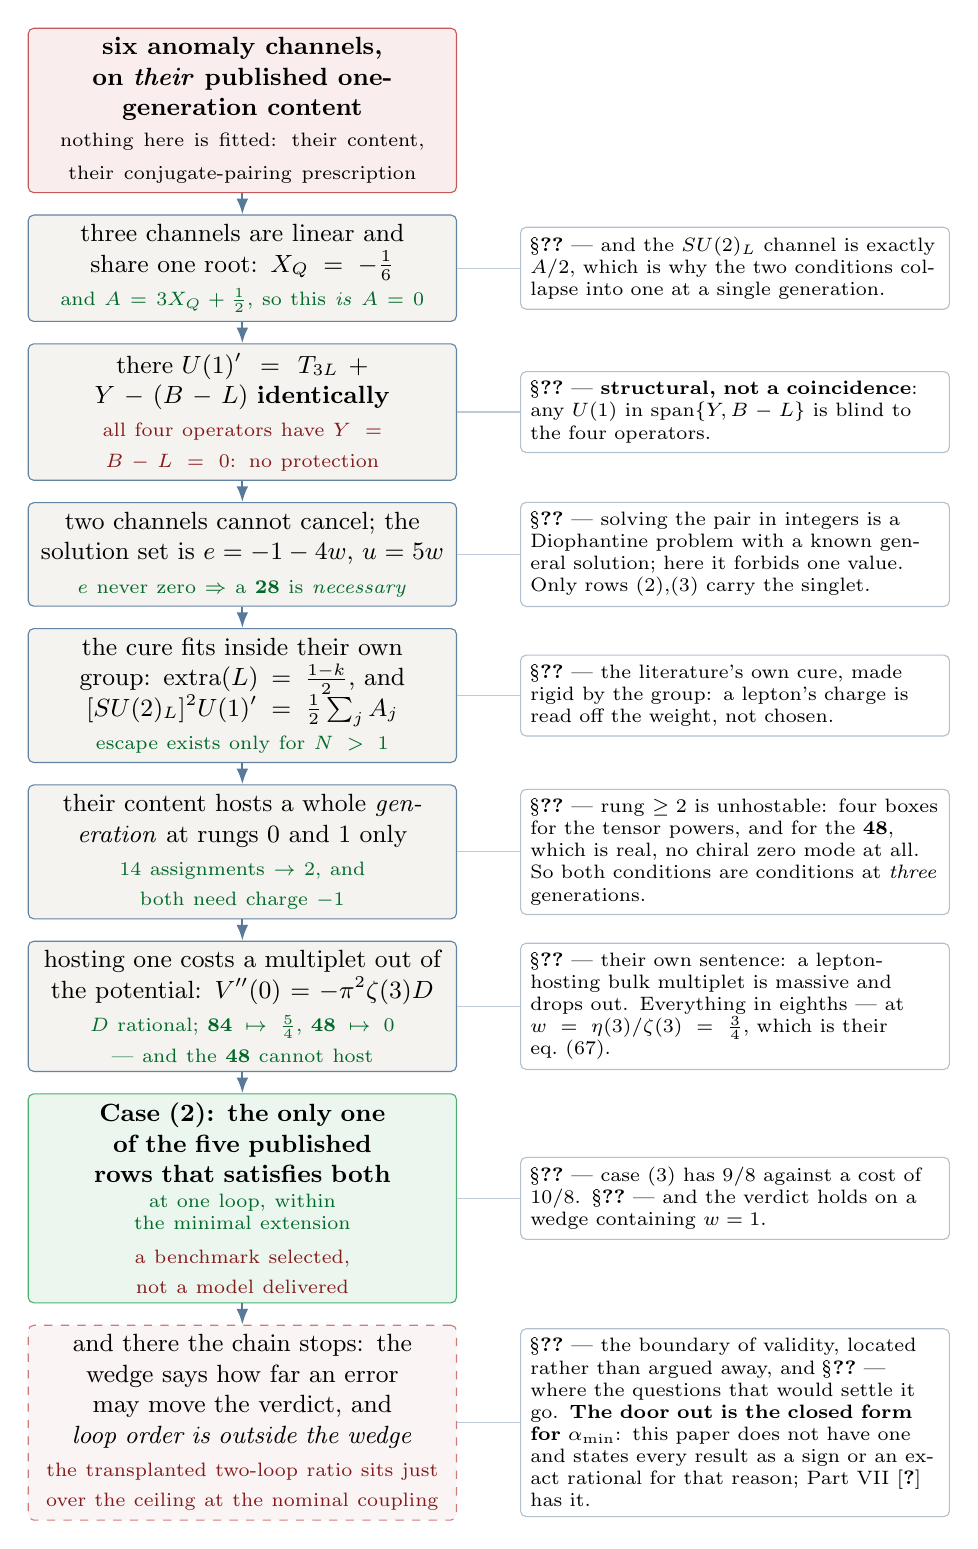
\begin{tikzpicture}[node distance=2.7mm, every node/.style={font=\small},
  bead/.style={draw=hdrblue!70,fill=softgrey,rounded corners=2pt,inner sep=3.4pt,
               minimum height=8mm,text width=52mm,align=center},
  root/.style={draw=warmred!75,fill=warmred!8,rounded corners=2pt,inner sep=3.4pt,
               minimum height=8mm,text width=52mm,align=center,font=\small\bfseries},
  gain/.style={draw=okgreen!70,fill=okgreen!8,rounded corners=2pt,inner sep=3.4pt,
               minimum height=8mm,text width=52mm,align=center},
  door/.style={draw=warmred!60,fill=warmred!5,rounded corners=2pt,inner sep=3.4pt,
               minimum height=8mm,text width=52mm,align=center,dashed},
  side/.style={draw=hdrblue!35,fill=white,rounded corners=2pt,inner sep=3.5pt,
               text width=52mm,align=left,font=\scriptsize},
  ar/.style={-{Latex[length=2mm]},hdrblue!75,thick}]

\node[root] (r) {six anomaly channels, on \emph{their} published one-generation content\\[3pt]
  {\normalfont\scriptsize nothing here is fitted: their content,\\[1pt] their conjugate-pairing
  prescription}};

\node[bead,below=of r] (x) {three channels are linear and share one root:
  $X_Q=-\tfrac16$\\[1pt]
  \scriptsize\textcolor{okgreen!75!black}{and $A=3X_Q+\tfrac12$, so this \emph{is} $A=0$}};

\node[bead,below=of x] (id) {there $U(1)'=T_{3L}+Y-(B-L)$ \textbf{identically}\\[1pt]
  \scriptsize\textcolor{warmred!75!black}{all four operators have $Y=B-L=0$: no protection}};

\node[bead,below=of id] (nu) {two channels cannot cancel; the solution set is
  $e=-1-4w$, $u=5w$\\[1pt]
  \scriptsize\textcolor{okgreen!75!black}{$e$ never zero $\Rightarrow$ a $\rep{28}$ is
  \emph{necessary}}};

\node[bead,below=of nu] (lad) {the cure fits inside their own group:
  $\mathrm{extra}(L)=\tfrac{1-k}{2}$, and $[\su2_L]^2U(1)'=\tfrac12\sum_jA_j$\\[1pt]
  \scriptsize\textcolor{okgreen!75!black}{escape exists only for $N>1$}};

\node[bead,below=of lad] (fit) {their content hosts a whole \emph{generation} at rungs $0$ and
  $1$ only\\[1pt]
  \scriptsize\textcolor{okgreen!75!black}{$14$ assignments $\to$ $2$, and both need charge $-1$}};

\node[bead,below=of fit] (d) {hosting one costs a multiplet out of the potential:
  $V''(0)=-\pi^2\zeta(3)D$\\[1pt]
  \scriptsize\textcolor{okgreen!75!black}{$D$ rational; $\rep{84}\mapsto\tfrac54$,
  $\rep{48}\mapsto0$ --- and the $\rep{48}$ cannot host}};

\node[gain,below=of d] (th) {\textbf{Case (2): the only one of the five published rows that
  satisfies both}\\[1pt]
  \scriptsize\textcolor{okgreen!75!black}{at one loop, within the minimal extension}\\[1pt]
  \scriptsize\textcolor{warmred!75!black}{a benchmark selected, not a model delivered}};


\node[door,below=of th] (lim) {and there the chain stops: the wedge says how far an error may move
  the verdict, and \emph{loop order is outside the wedge}\\[1pt]
  \scriptsize\textcolor{warmred!75!black}{the transplanted two-loop ratio sits just over the ceiling
  at the nominal coupling}};

\foreach \a/\b in {r/x,x/id,id/nu,nu/lad,lad/fit,fit/d,d/th,th/lim} \draw[ar] (\a) -- (\b);

\node[side,right=8mm of x]   (sx)  {\S\ref{sec:anom} --- and the $\su2_L$ channel is exactly
  $A/2$, which is why the two conditions collapse into one at a single generation.};
\node[side,right=8mm of id]  (sid) {\S\ref{sec:anom} --- \textbf{structural, not a coincidence}: any
  $U(1)$ in $\mathrm{span}\{Y,B-L\}$ is blind to the four operators.};
\node[side,right=8mm of nu]  (snu) {\S\ref{sec:anom} --- solving the pair in integers is a
  Diophantine problem with a known general solution; here it forbids one value. Only rows (2),(3)
  carry the singlet.};
\node[side,right=8mm of lad] (sla) {\S\ref{sec:ladder} --- the literature's own cure, made rigid by
  the group: a lepton's charge is read off the weight, not chosen.};
\node[side,right=8mm of fit] (sfi) {\S\ref{sec:ladder} --- rung $\ge2$ is unhostable: four boxes for
  the tensor powers, and for the $\rep{48}$, which is real, no chiral zero mode at all. So both
  conditions are conditions at \emph{three} generations.};
\node[side,right=8mm of d]   (sd)  {\S\ref{sec:vacuum} --- their own sentence: a lepton-hosting bulk
  multiplet is massive and drops out. Everything in eighths --- at $w=\eta(3)/\zeta(3)=\tfrac34$,
  which is their eq.~(67).};
\node[side,right=8mm of th]  (sth) {\S\ref{sec:vacuum} --- case (3) has $9/8$ against a cost of
  $10/8$. \S\ref{sec:repair} --- and the verdict holds on a wedge containing $w=1$.};

\node[side,right=8mm of lim] (slim) {\S\ref{sec:repair} --- the boundary of validity, located
  rather than argued away, and \S\ref{sec:open} --- where the questions that would settle it go.
  \textbf{The door out is the closed form for $\amin$}: this paper does not have one and states
  every result as a sign or an exact rational for that reason; Part~VII \cite{PartVII} has it.};

\foreach \a/\b in {x/sx,id/sid,nu/snu,lad/sla,fit/sfi,d/sd,th/sth,lim/slim}
  \draw[hdrblue!30] (\a) -- (\b);
\end{tikzpicture}
\caption{The chain, and it is one chain: every statement in this paper descends from the six anomaly
channels evaluated on \cite{KM25}'s own content. Left, the thread; right, what each link buys and
where it is done. Read top-down it is an \emph{obstruction} (the first three links, which depend on
no extension of ours), then a \emph{classification of the escapes} (the next two, which assume three
generations and their inventory), then a \emph{benchmark} (the next two). The green box selects the
row worth computing in full; it does not compute it. The dashed box is not a link but the edge of the
chain.}
\label{fig:chain}
\end{figure}

\paragraph{How to read it.} The chain is one chain, but its links are not all the same kind of
statement, and the paper is easier to judge if they are kept apart. \S\ref{sec:anom} is a
\emph{structural result about their published content}: six channels on the model as printed, and its
conclusion --- no protection, for an identity --- depends on no extension of ours.
\S\ref{sec:ladder} and \S\ref{sec:vacuum} are the \emph{minimal extension and its price}: they assume
three generations and their own inventory of representations, and a reader who enlarges that
inventory must re-run the first condition. \S\ref{sec:instrument} and \S\ref{sec:repair} are neither:
they are a \emph{diagnosis of the instrument}, including one column of their table we cannot
reproduce, and they exist so that the verdict can be judged rather than trusted.
\S\ref{sec:open} is what none of the three settles --- which is what the dashed box at the foot of
the figure marks: every box above it is exact at one loop and the statement in it is not, and the
first of the questions it opens is answered in Part~VII \cite{PartVII}.

\bridge{Everything below is arithmetic on someone else's equations, so the first question is which
equations: what is inherited from \cite{KM25} verbatim, and what has to be derived before it can be
used?}

% ===================================================================
\section{What is inherited, and what is computed}\label{sec:setting}

In gauge-Higgs unification the Higgs is the extra-dimensional component of a higher-dimensional
gauge field \cite{Manton,Hosotani}, so its potential is generated at one loop and is calculable. The
model of \cite{KM25} is six-dimensional $\su7$ on $S^1/\ZZ_2\times S^1/\ZZ_2$, a six-dimensional
extension of the five-dimensional $\su4$ gauge-Higgs unification that predicts
$\sin^2\theta_W=1/4$ at the compactification scale \cite{AHMN}. Its orbifold parities are their
eqs.~(11)--(13),
\[
P_6=\mathrm{diag}(+,+,+,-,-,-,-),\qquad
P_5=\mathrm{diag}(+,+,+,+,+,-,-),
\]
\[
P_5'=\mathrm{diag}(+,+,+,-,-,-,+),
\]
the Standard-Model fermions are localised at fixed points (their eqs.~(43)--(47)), and the bulk
carries 6D Dirac fermions in $\rep7$, $\rep{28}$, $\rep{48}$ and $\rep{84}$ whose only role is the
one-loop Higgs potential. Their Wilson-line vacuum leaves $\su3_C\times U(1)_{\rm em}$ together with
one extra abelian factor, their eq.~(79),
\begin{equation}\label{eq:u1p}
U(1)':\qquad T^{15}-\tfrac{\sqrt3}{3}T^{24}+\tfrac{\sqrt6}{3}T^{35}
=\tfrac12\,\mathrm{diag}(0,0,0,1,-1,1,-1),
\end{equation}
which they say must be broken by a $U(1)'$-charged 4D scalar on a fixed point. Their conclusion
states that \emph{``how the dangerous proton decay processes can be forbidden, for instance, by some
symmetries \dots are left for our future work.''} This paper answers that.

Three properties of their construction are inherited verbatim and used throughout. (i) The Standard
Model fermions are \emph{not} embedded in the multiplets of their Table~1 --- of the bulk fermions of
their \S3.2 they write that \emph{``these 6D fermions have nothing to do with the SM quarks and
leptons, namely the SM fermions are not embedded in \underline{these} $\su7$ multiplets.''} Their
leptons are elsewhere \emph{in the bulk}, in a $\rep{21}$ whose parity they fix by hand in their
eq.~(43); their quarks are 4D fields on a fixed point, for their own stated reason, that the
fractional hypercharges of quarks are not on the lattice a tensor product of $\rep7$s generates. That
distinction is the whole mechanism of \S\ref{sec:ladder}: the escape moves a lepton generation out of
a multiplet that is \emph{not} in their Table~1 and into one that is, and that is why it has a price.
(ii) Unwanted bulk zero modes are lifted by 4D fermions conjugate to them with Dirac masses on the
fixed points, the sentence after their eq.~(76); a vector-like pair contributes nothing to any
anomaly, which we verify rather than assume (200 random pairs, largest change $0$). (iii) A bulk
multiplet that hosts leptons must be massive, and a massive bulk fermion's potential carries
$e^{-M\pi R}\sim e^{-O(10)}$ and is dropped --- their own sentence below eq.~(79). Point (iii) is
what turns a group-theoretic escape into a bill charged against their Table~1, and it is their
sentence, not our inference.

Everything else is computed. To make that credible we first rebuilt the whole of their \S3 from
their own equations rather than trusting it: their structure constants (their eq.~(54)) come out
$13/13$ exact, and the one they omit, $f^{48,44,45}$, is exactly zero, which is \emph{why} the
$U(1)$ is absent from their list; the Kaluza-Klein spectrum on the adjoint has Wilson-line charges
$\{0,\pm\tfrac12,\pm1\}$ with multiplicities $26,20,2$, cross-checked by pure representation theory
($\rep3+\rep1+10\cdot\rep2+24\cdot\rep1$ under the $\su2$ generated by $T^{44}$); their gauge
potential eq.~(68) is rebuilt with its coefficient $7=4+3$ identified ($4$ from $A_\mu$ on the two
colour-singlet doublets, $3$ from $A_5,A_6$ on the six coloured states, and no ghost anywhere);
their eq.~(67) is \emph{proved} rather than sampled; and all four branchings (41), (57), (69), (70)
are derived from (11)--(13), with hypercharges and all three parities.

Their eq.~(68) is also derived from the group theory, and not only from their own eq.~(62), which is
a different and weaker statement. Because their Wilson line touches only indices $5$ and $7$, and
both $P_5P_5'$ and $P_6$ take the same value on those two, the Wilson-line charge and the two
parities are simultaneously diagonal --- so every one of the $48$ adjoint generators carries a
definite $(q,P_5P_5',P_6)$, and eq.~(68) must be a sum over that table. It is. Writing $a$ for the
weight of a $P_6=+1$ pair and $b$ for a $P_6=-1$ pair, the two rows with no $P_6=-1$ pairs fix
$a=2$ independently of each other --- a redundancy that could have failed and does not --- and the
remaining row then gives $b=\tfrac12$. All three coefficients follow: $2$, $4$, and
$7=2\cdot2+6\cdot\tfrac12=4+3$, which is the split their own text states and never derives.

One of those rebuilds settles a relation they import rather than derive. Their eq.~(81),
$m_W^2=\alpha^2/4R_5^2$, is introduced with the words \emph{``the W boson mass in 5D $\su4$ GHU is
given by''} --- a different model --- and their eq.~(82), the whole $1/R_5$ column of their Table~1
and the constant in \eqref{eq:K} below all rest on it. It is also a theorem of their own $\su7$.
Their eq.~(41) puts $\su2_L$ on indices $4,5$, so $W^\pm$ are the raising and lowering combinations
there; under the shift operator $M^{ac}=f^{a,44,c}$ of their eq.~(53) those directions carry
Wilson-line charge $\tfrac12$, not the $1$ carried by the only two other charged modes, so the
lightest tower gives $m_W=\alpha/2R_5$ from their eq.~(54) alone. The control that had to fire does:
the charge-$1$ modes exist --- had $W$ been one of them their eq.~(82) would carry a factor $2$ ---
and the photon direction of their eq.~(78) comes out exactly neutral, so it stays massless.

\begin{observation}[a partial match is more dangerous than none]
The obvious Cartan for their generator labels --- the nested chain
$\su2\subset\su3\subset\dots\subset\su7$, whose diagonal generators sit at $3,8,15,24,35,48$, where
theirs sit --- reproduces \emph{eleven of the thirteen} constants of their eq.~(54) and fails on the
three diagonal ones. It reads as ``their paper has two errors in the diagonal sector.'' It is not:
the guess is wrong, refuted by their own eqs.~(78) and (79), and it puts $T^{48}$ --- which they
state commutes with the Wilson line --- on a generator that does not.
\end{observation}

Two facts about their \S3.2 that they do not state but that it needs came out of the rebuild. First,
their $\rep{28}$ is $\mathrm{Sym}^2(\rep{\bar7})$, the \emph{conjugate}: read as
$\mathrm{Sym}^2(\rep7)$ its eq.~(69) matches $2/4$, with every parity right and two hypercharges
negated, and as $\mathrm{Sym}^2(\rep{\bar7})$ it matches $4/4$. The test discriminates --- the
$\rep{84}$ fits $\mathrm{Sym}^3(\rep7)$ at $10/10$ and $\mathrm{Sym}^3(\rep{\bar7})$ at $1/10$. It
is invisible to $V_{\rm eff}$, which uses only the $\su2_L$ label and the product
$\eta\eta'P_5P_5'$, so it is a datum and not a defect. Second, and load-bearing: their Wilson line
(their eq.~(77)) is the identity except on indices $5$ and $7$, and $P_5P_5'$ takes the \emph{same}
value $-1$ on those two indices. Were it otherwise, the Wilson-line charge eigenbasis
$u,v=(5\pm7)/\sqrt2$ would not be a parity eigenbasis, and their eq.~(72), which depends on the
single product $\eta P_5\eta'P_5'$, would not be well defined.

\bridge{With their section 3 derived rather than assumed, the extra $U(1)$ can be interrogated on
its own terms. The first question is what anomaly cancellation leaves free.}

% ===================================================================
\section{All six channels, and what they force}\label{sec:anom}

Write $X_Q$ for the $U(1)'$ charge of the brane quark doublet. Their eq.~(47) is
$Y_u\,\bar q_L\tilde A_5 u_R+Y_d\,\bar q_L A_5 d_R$, and the $A_5$ zero mode carries
$\mathrm{extra}(H)=+1/2$, so $\mathrm{extra}(u_R,d_R)=X_Q\pm\tfrac12$ and the quark Yukawas fix
everything but $X_Q$ itself. The four dimension-6 $|\Delta B|=1$ operators then carry a single
$U(1)'$ charge
\begin{equation}\label{eq:A}
A=3X_Q+\tfrac12 .
\end{equation}
The $U(1)'$ forbids all four \emph{except} at the single point $A=0$, i.e.\ $X_Q=-1/6$.

Evaluating all six anomaly channels on their published one-generation content, with their own
conjugate-pairing prescription applied so that lifted zero modes contribute nothing:

\begin{center}\small
\begin{tabular}{lll}
\toprule
\rowcolor{hdrblue!12}
channel & coefficient, as a polynomial in $X_Q$ & vanishes at\\
\midrule
$[\su3_C]^2\,X$ & $0$ & every $X_Q$\\
\rowcolor{amber!13}
$[\su2_L]^2\,X$ & $\tfrac32X_Q+\tfrac14$ & $X_Q=-1/6$\\
\rowcolor{amber!13}
$X^2Y$ & $-3X_Q-\tfrac12$ & $X_Q=-1/6$\\
\rowcolor{amber!13}
$XY^2$ & $-\tfrac32X_Q-\tfrac14$ & $X_Q=-1/6$\\
\rowcolor{warmred!13}
$X\cdot\mathrm{grav}^2$ & $1$ & \textbf{never}\\
\rowcolor{warmred!13}
$X^3$ & $1$ & \textbf{never}\\
\bottomrule
\end{tabular}
\end{center}

All three constraining channels are \emph{linear} in $X_Q$ and all three have the same root. Note
that the first of them is $\tfrac32X_Q+\tfrac14=\tfrac12\big(3X_Q+\tfrac12\big)=A/2$: the
$\su2_L$ anomaly \emph{is} half the proton-operator charge. That is the one-generation case of
Proposition~\ref{prop:identity} below, and it is why the two conditions collapse into one here.

\begin{keyeq}
\textbf{Three independent channels force $X_Q=-1/6$, which by \eqref{eq:A} is exactly $A=0$ --- the
one point at which the $U(1)'$ stops forbidding proton decay.} And at that point, on every field of
the theory,
\[
U(1)'=T_{3L}+Y-(B-L)\qquad\text{identically},
\]
while all four dimension-6 operators have $Y=0$ \emph{and} $B-L=0$. Any $U(1)$ in that span is blind
to them. The failure is structural, not a coincidence of a fitted charge.
\end{keyeq}

\emph{Controls.} The four pure-Standard-Model channels vanish identically, so one generation with no
$\nu_R$ is anomaly free and the content bookkeeping is sound; $T(\text{fund})=\tfrac12$ comes
\emph{out} of the Cartan sum for both $\su2$ and $\su3$ instead of being put in; the derived
$Y=(0,0,0,\tfrac12,\tfrac12,-1,0)$ is traceless and reproduces the hypercharges of their eq.~(41);
and the whole calculation was re-derived independently under Sage from the $A_6$ Weyl character
ring with symbolic $X_Q$. The Sage control \emph{fired}: the $\rep{48}$ had first been built from
its $42$ roots only, with the six-state Cartan omitted. Those states are chargeless, so no anomaly
number moved --- but the zero-mode counts were wrong, and would have propagated.

The two channels that cannot cancel are the interesting ones. $X\cdot\mathrm{grav}^2$ and $X^3$
both come out equal to the constant $1$, so cancelling them requires additional
Standard-Model singlets $x_i$ with
\[
\textstyle\sum_i x_i=-1\quad\text{and}\quad\sum_i x_i^3=-1,
\]
two independent conditions. The minimal solution is one singlet of charge $-1$: a right-handed
neutrino. Among their own representations, the Standard-Model singlets with $Y=0$ are exactly the
pure index-7 components --- a charge $m/2$ needs $m$ boxes --- so
\[
\rep7\to\mp\tfrac12,\qquad \rep{28}\to\mp1,\qquad \rep{84}\to\mp\tfrac32,\qquad \rep{48}\to 0 .
\]
Minimality is not needed, and it is worth not leaning on it. Solving a pair of gravitational and
cubic $U(1)$ conditions in integers is a Diophantine problem with a known general
solution \cite{CDF}, and on the finite charge set their representations supply it collapses to two
lines. Write $u,w,e$ for the \emph{net} numbers of singlets at $\pm\tfrac12$, $\pm\tfrac32$ and
$\pm1$. The conditions read $u+3w+2e=-2$ and $u+27w+8e=-8$; subtracting them gives $24w+6e=-6$, so
the entire solution set is the one-parameter family
\[
e=-1-4w,\qquad u=5w ,
\]
a family of exactly the shape \cite{CDF} guarantees. What is particular to their model is which
value it forbids.

\begin{keyeq}
\textbf{Hence $e$ is never zero, and the $\rep{28}$ is not the cheapest way to cancel the two
channels but the only one} --- $e=0$ would require $w=-\tfrac14$. No number of $\rep7$s and
$\rep{84}$s, at any parities, cancels them. Imposing this on their Table~1, only cases \textbf{(2)}
and \textbf{(3)} can: case (1) has a $\rep{28}$ but at a parity that leaves no singlet zero mode, and
cases (4) and (5) contain no $\rep{28}$ at all.
\end{keyeq}

This is a constraint on \emph{their} model, and it is not stated in their paper --- which is what one
would expect, since it only becomes visible once the proton-decay question they set aside is taken up.
It is also the half of this paper's conclusion that nothing downstream can disturb: it is a statement
about which components exist in their eqs.~(69) and (70) with their parities, and no repair of the
\emph{potential} can reach it. That will matter in \S\ref{sec:repair}.

\bridge{So at one generation the surviving symmetry cannot supply the protection, and the reason is
an identity rather than an accident of a fitted charge. The literature has a cure for exactly this;
does it fit inside their own group?}

% ===================================================================
\section{A ladder inside their own $\su7$}\label{sec:ladder}

The disease --- a gauged $B-L$ (or anything in $\mathrm{span}\{Y,B-L\}$) failing to forbid the
$B-L$-conserving proton operators --- is old, and so is its cure: make the abelian charge
\emph{family-dependent}, $B-x_iL$ with $\sum x_i=3$ and $x_i\neq1$ \cite{FamilyU1}. In \cite{KM25}
a lepton's charge is not free data: the leptons come from a bulk multiplet and $U(1)'$ is a fixed
generator of $\su7$, so the charge is read off the weight. The question is whether the cure survives
that rigidity.

Demand that a component of an $\su7$ tensor be a colour singlet, an $\su2_L$ doublet member, and
$Y=-1/2$. With $Y=(0,0,0,\tfrac12,\tfrac12,-1,0)$ per index, the non-weak part must carry $Y=-1$:
exactly one index $6$, and any number $k$ of index $7$.

\begin{center}\small
\begin{tabular}{cclcll}
\toprule
\rowcolor{hdrblue!12}
$k$ & boxes & $L$ & $\mathrm{extra}(L)$ & $e_R$ (their eq.~(46): $5\leftrightarrow7$) &
$\mathrm{extra}(L)+\mathrm{extra}(e^c)$\\
\midrule
$0$ & 2 & $(5,6)$ & $\phantom{-}1/2$ & $(6,7)$ & $1/2$\\
\rowcolor{amber!14}
$1$ & 3 & $(5,6,7)$ & $\phantom{-}0$ & $(6,7,7)$ & $1/2$\\
$2$ & 4 & $(5,6,7,7)$ & $-1/2$ & $(6,7,7,7)$ & $1/2$\\
\bottomrule
\end{tabular}
\end{center}

\noindent
The rung index is $k$, the number of index-7 boxes --- \emph{not} the total number of boxes, which
is $k+2$. The shaded row is the one that matters below.

\begin{keyeq}
\[
\mathrm{extra}(L)=\frac{1-k}{2}
\]
--- a ladder spaced by $1/2$ and indexed by how many index-7 boxes the multiplet carries. Not free,
and not unique: exactly what family dependence needs.
\end{keyeq}

\emph{Controls.} Rung 0 reproduces their own $L=\rep{21}^{56}$, i.e.\ their eq.~(43), with nothing
put in by hand; and $\mathrm{extra}(L)+\mathrm{extra}(e^c)=\tfrac12$ --- the Higgs's own charge ---
on \emph{every} rung, so the charged-lepton Yukawa closes at each one, since it comes from the 6D
gauge coupling inside a single multiplet.

\begin{proposition}[the identity that decides it]\label{prop:identity}
For $N$ generations with proton-operator charges $A_j=3a_j+l_j$,
\[
[\su2_L]^2\,U(1)'=\tfrac12\sum_j A_j\qquad\text{exactly}.
\]
\end{proposition}

\noindent
It is obtained by summing the $\su2_L$ anomaly state by state over $N$ generations and comparing
with $\sum_jA_j$; the $N=1$ case is the entry $\tfrac32X_Q+\tfrac14=A/2$ of the table in
\S\ref{sec:anom}, which is where it can be read off directly.

Anomaly cancellation demands $\sum_j A_j=0$; proton protection demands $A_j\neq0$ for every $j$. At
$N=1$ these are the \emph{same equation}, which is the entire content of \S\ref{sec:anom}. At $N=3$
they are not: a sum vanishes with no term vanishing. \textbf{The escape is real, and it exists only
for $N>1$.} This is \cite{FamilyU1}'s $\sum x_i=3$, $x_i\neq1$ in their variables.

Keeping the brane-quark charge family-universal --- which is what an unrestricted renormalisable CKM
structure requires \emph{before} $U(1)'$ is broken, since a family-dependent $a_j$ forbids the
off-diagonal quark Yukawas there; afterwards, operators dressed with $\langle\varphi\rangle$ can
regenerate mixing, so this is a choice of the minimal extension and not a theorem --- gives
$a=-(\sum l)/9$ and
$A_j=l_j-\bar l$, so \emph{protection holds iff no generation sits at the mean}. Imposing all six
channels with right-handed neutrinos drawn from the singlet ladder, \textbf{14 assignments of (rung
set, $X_Q$) survive}, each naming the representation and parity of the neutrinos it needs. The
control that had to fire does: the family-universal rungs $(\tfrac12,\tfrac12,\tfrac12)$ return
$a=-1/6$ and $A_j=0$, recovering \S\ref{sec:anom} as a special case.

Whether the orbifold \emph{keeps} such a generation is a separate question, and their eqs.~(37)--(40)
answer it: a zero mode exists iff $p_5p_5'=\eta\eta'$, with chirality $g=-\eta p_5$. Demanding $L$
left-handed and $e_R$ right-handed:

\begin{center}\small
\begin{tabular}{clp{0.52\textwidth}}
\toprule
\rowcolor{hdrblue!12}
representation & rung $k$ & hosted at\\
\midrule
$\rep{21}$, $\rep{28}$ & 0 & $(\eta,\eta')=(-1,+1)$ --- their own eq.~(43)\\
\rowcolor{warmred!13}
$\rep{35}=\Lambda^3$ & 1 & \textbf{never} --- $e_R=(6,7,7)$ needs a repeated index, which an
antisymmetric tensor has not\\
\rowcolor{amber!16}
$\rep{84}$ & 1 & $(\eta,\eta')=(+1,+1)$\\
\rowcolor{warmred!13}
$\rep{48}=\text{adj}$ & 0, 2 & \textbf{never} --- it carries four lepton doublets, but
$\langle A_5\rangle$ takes none of them to a charged-lepton singlet\\
\bottomrule
\end{tabular}
\end{center}

\begin{keyeq}
\textbf{And an $\rep{84}^{(+,+)}$ is already in every single row of their Table~1}, introduced for
the Higgs potential and for nothing else. The multiplet that would host a third, inequivalent lepton
generation is not a new ingredient.
\end{keyeq}

Their own tensors then decide which rungs exist at all, and it is a short count. A rung-$k$ doublet
is the component $(5,6,7^k)$, so $2+k$ boxes, and its partner $e_R=(6,7^{k+1})$ must sit in the
\emph{same} multiplet or the Yukawa of their eq.~(46) does not close. Rung $0$ needs two boxes: the
$\rep{21}$ or the $\rep{28}$. Rung $1$ needs three, and by the row above only the $\rep{84}$ of them
survives. Rung $2$ and above need four boxes or more, and no such tensor power is in their paper.

That last sentence is not the whole exclusion, and the part it misses is load-bearing. The
$\rep{48}$ is not a tensor power at all, so a box count does not reach it --- and it sits in three of
their five rows. Counted directly, the adjoint \emph{does} carry a lepton doublet: the pair
$(7,\bar4),(7,\bar5)$, with $Y=-\tfrac12$ and $\mathrm{extra}=-\tfrac12$, which is rung $2$. It
survives the projection in a $\rep{48}^{(+,+)}$, and the test that says so rejects $8$ of the $10$
states at $|q|=\tfrac12$, so it is not vacuous. Its charged-lepton partner would need
$(Y,\mathrm{extra})=(-1,-1)$, which is nowhere in their content: absent from the $\rep{48}$, and as a
tensor it is $(6,7^3)$, four boxes.

But the partner is the wrong place to look, and no localised field can rescue this.

\begin{proposition}[a real representation under diagonal $\pm1$ parities furnishes no chiral
generation]\label{prop:real}
Let the orbifold parities $P_5,P_5'$ act diagonally on the indices of the fundamental, so that a
component of a bulk multiplet survives in the multiplet of parities $(\eta,\eta')$ iff
$P_5P_5'=\eta\eta'$ and then carries $4$D chirality $-\eta\,P_5$ (their eqs.~(37)--(40)). Then for a
\emph{real} representation the surviving spectrum is vector-like, with no chiral state at either
choice of $(\eta,\eta')$.
\end{proposition}

\begin{proof}
For the adjoint $\rep7\otimes\rep{\bar7}-\rep1$ the conjugate of the component $(i,\bar\jmath)$ is
$(j,\bar\imath)$, which lies in the \emph{same} multiplet. Since the parities are diagonal,
$P_5P_5'(j,\bar\imath)=p_jp_i=P_5P_5'(i,\bar\jmath)$ and
$P_5(j,\bar\imath)=P_{5,j}P_{5,i}=P_5(i,\bar\jmath)$: the two survive together and with the same
chirality. In an all-left-handed convention the two surviving Weyl fields transform in conjugate
gauge representations and therefore admit a gauge-invariant Dirac mass --- and their own
prescription, a conjugate fixed-point fermion against each unwanted zero mode, supplies one. The
argument uses no property of the Wilson line and none of the particular \emph{values} of these
parities --- but it does use that they are $\pm1$ and diagonal, which is what makes the projection
commute with conjugation, and that hypothesis is not free. A $\ZZ_3$ projection has complex
eigenvalues, breaks the pairing, and is precisely how the literature obtains chiral families from an
adjoint \cite{GMN}. Their eqs.~(37)--(40) are $\ZZ_2$, so that escape is closed in their model and
not in general. \qed
\end{proof}

\noindent Counted on their content: a $\rep{48}^{(+,+)}$ has $18$ surviving states and \textbf{all
$18$} are so paired; a $\rep{48}^{(+,-)}$, $24$ of $24$. \textbf{Zero chiral states, either way.} The
doublet arrives already married to its own conjugate, so there is nothing for a localised partner to
complete: a brane field would supply the $e_R$, and the defect is one step earlier.

\emph{Control that had to separate two things, and does.} If $\mathrm{Sym}^2$ and $\mathrm{Sym}^3$
came out vector-like too, this would be measuring the orbifold rather than the reality of the
representation --- and their model could have no chiral matter at all. They do not: the $\rep{28}$
leaves $10$ unpaired states and the $\rep{84}$ leaves $34$. The criterion distinguishes exactly what
it claims to.

This also explains a sentence of theirs we had read as a stipulation. Their $\rep7$, $\rep{28}$,
$\rep{48}$ and $\rep{84}$ are introduced with the Higgs potential as their only role; for the
$\rep{48}$ that is not a modelling choice but the only thing a real representation can do here. And
it closes the ladder without a residue: no real representation furnishes a chiral generation on this
orbifold, so the box count and the reality condition between them cover every multiplet their model
contains.

\paragraph{Why this is not merely a tidier proof.} Donating a $\rep{48}^{(+,+)}$ would cost
$D=6-\tfrac34\cdot8=0$ \textbf{exactly} (\S\ref{sec:vacuum}), and case (3) holds three of them. Had
the adjoint been able to host the escape, case (3) would pay nothing, keep its $9/8$, survive, and
the conclusion of \S\ref{sec:vacuum} would fail outright --- and the assignment that would have used
it, $l=(\tfrac12,\tfrac12,-\tfrac12)$ at $X_Q=-1/18$, is one of the fourteen that cancel all six
channels, so anomalies do not forbid it, the charge $-1$ is on the bulk lattice, and their own quarks
are already brane fields. Every gate we could think of was open except one. The exclusion of the
$\rep{48}$ is therefore a step of the argument and not an aside, and the step is the reality of the
representation.

\begin{keyeq}
\textbf{Twelve of the fourteen assignments therefore do not fit inside their own content, and
exactly two do}: $l=(\tfrac12,\tfrac12,0)$ at $X_Q=-1/9$, and $l=(\tfrac12,0,0)$ at $X_Q=-1/18$.
\textbf{Both of them require a Standard-Model singlet of charge $-1$} --- so the requirement of
\S\ref{sec:anom}, derived on their published \emph{one}-generation content, is still the requirement
on the minimal \emph{three}-generation extension.
\end{keyeq}

The first is the minimal change --- two generations in $\rep{21}$s, the third in an
$\rep{84}^{(+,+)}$, with $A=(\tfrac16,\tfrac16,-\tfrac13)$, all non-zero. The second puts two
generations in $\rep{84}^{(+,+)}$s and one in a $\rep{21}$, with $A=(\tfrac13,-\tfrac16,-\tfrac16)$.
They differ in how many $\rep{84}$s leave the Higgs potential, which is the subject of the next
section, and \S\ref{sec:vacuum} settles both.

\bridge{The escape is consistent at the level of anomalies, charges, Yukawas and zero modes. It is
not free: by their own sentence, a lepton-hosting multiplet leaves the Higgs potential. What does
that cost?}

% ===================================================================
\section{The bill, in eighths}\label{sec:vacuum}

Electroweak symmetry breaking in this model requires $\alpha=0$ to be a \emph{maximum} of
$V_{\rm eff}$: $\alpha=0$ is the symmetric point ($m_W=\alpha/2R_5=0$) and $\alpha=1$ is their
Fig.~1 case, so the vacuum must sit strictly inside. Expanding their eqs.~(68) and (72)--(76) at
the origin, every term is $m c^2\sum_n s^n/n^3$ and those two series are exactly $\zeta(3)$ and
$-\tfrac34\zeta(3)$. Hence

\begin{keyeq}
\[
V''(0)=-\pi^2\zeta(3)\,D,\qquad
D=\sum_{s=+1}m c^2-\tfrac34\sum_{s=-1}m c^2\quad\in\mathbb{Q},
\]
and electroweak symmetry breaking is possible \textbf{iff $D>0$}.
\end{keyeq}

\paragraph{What $D$ decides, and what it does not.} $D$ is the curvature at \emph{one point}. It says
the symmetric point is a maximum, and that is all it says: by itself it does not fix where the global
minimum falls, whether it falls anywhere phenomenologically useful, the curvature there, or whether a
competing minimum exists elsewhere in the period. Two of those four are measurable without predicting
anything absolute, and they are measured. On the fifteen configurations the verdict is actually read
from --- their five rows, and the same five after donating one and after donating two
$\rep{84}^{(+,+)}$ --- the sign of $D$ coincides with the existence of an interior minimum in
$15$ of $15$, and \emph{no} configuration has more than one interior local minimum on a grid over the
whole period. Using the sign as the verdict is therefore not an unchecked leap. It is also not a
theorem, and we do not call it one: a content outside this set could in principle carry $D>0$ with
its minimum pushed to the edge. The other two --- where the minimum falls in GeV, and the curvature
there --- stay out of reach on purpose, because \S\ref{sec:instrument} does not reproduce their
$\amin$ column and no absolute number is claimed for modified content. That is exactly why the
verdict is a \emph{sign}.

\textbf{One thing that reads here as an empirical margin is not one, and it is worth saying where it
becomes a theorem.} Every multiplet in the table below contributes a $D$ in $\tfrac14\ZZ$ while the
gauge sector contributes $-27/8$, which is not, so
\[
  D=\frac{-27+2k}{8},\qquad k\in\ZZ,
\]
with an odd numerator always: $D$ cannot vanish, and $|D|\ge\tfrac18$. Part~VII \cite{PartVII} proves
that and reads the consequences off it; here it does one thing, and it is the thing $15$ of $15$ was
standing in for --- the curvature at the symmetric point is never marginal in this class, so the sign
is always defined. It also puts case~(3)'s failure in its place: $9/8-10/8=-1/8$ is the negative
value of \emph{smallest possible modulus}, so the row that loses electroweak symmetry breaking loses
it by the narrowest margin the quantisation allows.

\emph{Control, in its sharp form.} A closed form cannot equal a truncated sum, so instead of
tolerating the difference we \emph{predict} it from the tail of $\zeta(3)$; it matches to better
than $2\,\%$ on all five rows. A second control had to fire and did: the criterion calls the
gauge-only content dead --- their Fig.~1, reproduced exactly at $\amin=1.00000$ --- and their own
unreduced rows alive. A third is recorded as a failure: the first version of the guard called
$\alpha\to0$ ``EWSB survives'', when $\alpha=0$ is the symmetric point and is also unbroken.

\begin{center}\small
\begin{tabular}{lr@{\qquad}lr}
\toprule
\rowcolor{hdrblue!12}
multiplet & $D$ & multiplet & $D$\\
\midrule
gauge sector & $-27/8$ & $\rep{28}^{(+,+)}$ & $2$\\
$\rep7^{(+,+)}$ & $-3/4$ & $\rep{28}^{(+,-)}$ & $1/4$\\
$\rep7^{(+,-)}$ & $1$ & \cellcolor{hdrblue!16}$\rep{48}^{(+,+)}$ &
\cellcolor{hdrblue!16}$\mathbf{0}$\\
& & \cellcolor{amber!18}$\rep{84}^{(+,+)}$ & \cellcolor{amber!18}$\mathbf{5/4}$\\
\bottomrule
\end{tabular}
\end{center}

The $\rep{48}$ contributes \emph{exactly zero} at the origin --- it cannot help destabilise the
symmetric point at all --- and each $\rep{84}^{(+,+)}$ is worth exactly $5/4$.

\begin{figure}[t]
\centering
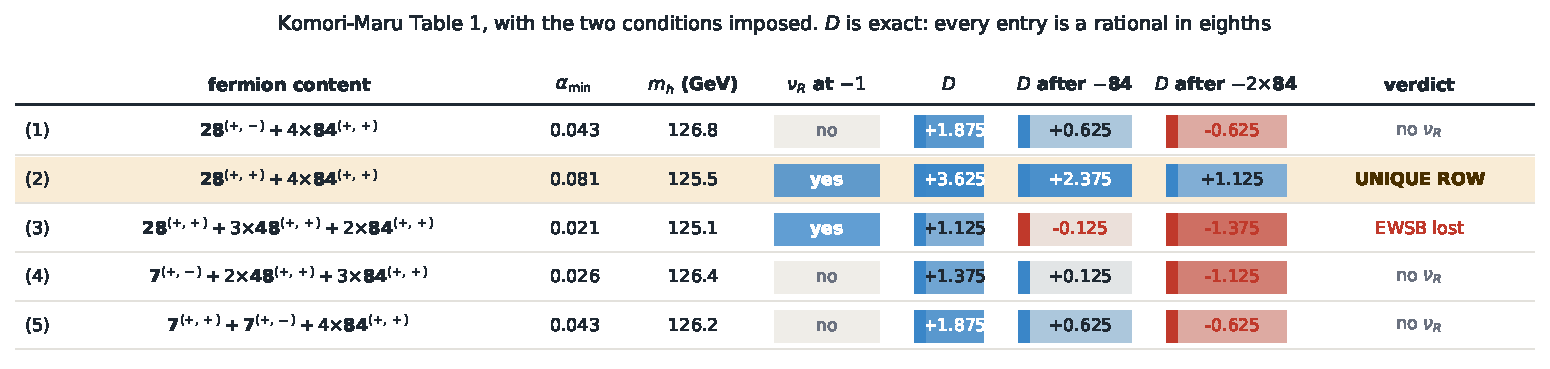
\includegraphics[width=\textwidth]{fig_table1_verdicts.pdf}
\caption{Table~1 of \cite{KM25} with the two conditions of this paper imposed. The $\nu_R$ column is
\S\ref{sec:anom}: which rows contain a Standard-Model singlet of $U(1)'$ charge $-1$, a statement
about which components exist and therefore immune to everything in \S\ref{sec:instrument}. The two
$D$ columns are \S\ref{sec:vacuum}, before and after donating one $\rep{84}^{(+,+)}$ to host the
third lepton generation; every entry is an exact rational in eighths, and the coloured bar carries
the sign, which is the whole content. Case (3) --- the row \cite{KM25} single out as
\emph{particularly interesting} --- has only $9/8$ to spend against a cost of $10/8$. Generated by
\texttt{make\_figures\_su7.py} from the archived \texttt{su7\_repair\_space.json}.}
\label{fig:verdicts}
\end{figure}

Write $\lambda$ for a uniform rescaling of the whole fermion sector, so that $\lambda=1$ is their
own normalisation, and $\lambda_{\rm crit}$ for the value at which a reduced row changes verdict.

\begin{center}\small
\begin{tabular}{lrrrp{0.34\textwidth}}
\toprule
\rowcolor{hdrblue!12}
case & $D$ theirs & $D$ after donating an $\rep{84}$ & $\lambda_{\rm crit}$ & verdict\\
\midrule
(1) & $15/8$ & $5/8$ & $0.8438$ & EWSB survives\\
\rowcolor{amber!12}
\textbf{(2)} & $\mathbf{29/8}$ & $\mathbf{19/8}$ & $\mathbf{0.5870}$ & \textbf{survives, largest
margin of the five}\\
\rowcolor{warmred!12}
\textbf{(3)} & $\mathbf{9/8}$ & $\mathbf{-1/8}$ & $\mathbf{1.0385}$ & \textbf{EWSB LOST}: the
symmetric point becomes the vacuum\\
(4) & $11/8$ & $1/8$ & $0.9643$ & survives, barely\\
(5) & $15/8$ & $5/8$ & $0.8438$ & EWSB survives\\
\bottomrule
\end{tabular}
\end{center}

\begin{keyeq}
\textbf{Donating an $\rep{84}$ costs exactly $5/4=10/8$, and case (3) only has $9/8$ to spend.} It
goes to $-1/8$, the sign flips, and $\alpha=0$ becomes a genuine minimum. Everything is in eighths
and nothing is numerical.

Combining with \S\ref{sec:anom}: only rows (2) and (3) can supply the required $\nu_R$; of those,
(3) loses electroweak symmetry breaking when it pays for the escape. \textbf{Case (2) is the only one
of the five published rows that satisfies both necessary conditions at once --- within the minimal
extension considered, and at the level of the one-loop curvature} (Fig.~\ref{fig:verdicts}). That is
a strong filter and not a working construction: it is not the claim that case (2) \emph{works}. It is
also the row with the
lowest compactification scale of the five, $1/R_5=2.0$~TeV, the most accessible one. The row they
single out, case (3) at $7.5$~TeV, is the one that cannot.
\end{keyeq}

\noindent
\textbf{And ``worth computing'' is a smaller claim than it may look, because part of that
computation now exists.} Part~VII \cite{PartVII} minimises the reduced potential and finds that the
naively donated row does \emph{not} stay inside the original $125$--$127$~GeV window --- none of the
five does. Case~(2) remains the benchmark this paper selects because the selection is made at the
curvature, where it is exact, and because it is the lowest of the four rows that still break; what
has not been built, and what the row would need in order to be a model, is the completion
\S\ref{sec:open} ends on: the localised terms and the scalar sector. The next problem is therefore
not to minimise $\rep{28}+3\times\rep{84}$ once more. It is to construct the theory around case~(2).

\paragraph{Exact is not the same as unconditional, and the condition is one equation of theirs.}
The $3/4$ in $D$ is $\eta(3)/\zeta(3)=1-2^{1-3}$, and the $3$ is the $n^3$ two lines above: the
potential goes as $1/n^5$ and two derivatives in $\alpha$ bring down $n^2$. That $1/n^5$ is their
eq.~(67), proved in \S\ref{sec:instrument} and not assumed here. Writing
$w$ for that ratio, $D_i-\text{cost}$ is linear in $w$ and the verdict holds exactly on
$w\in[74/99,\,118/151)$. Of the admissible values $w=1-2^{1-p}$ only $w=3/4$ lies inside: at $1/2$
case (3) survives too and the row is not unique, and at $7/8$ and above \emph{no} row survives and
the minimal extension dies outright. So the proof of their eq.~(67) carries this section as well as
\S\ref{sec:instrument}. It is not a fragility --- $w$ is quantised and its admissible neighbours are
nowhere near the window --- but it is a dependency, and it is stated here rather than left implicit.

\paragraph{Both conditions are conditions on the same three-generation extension.} The $\nu_R$
requirement of \S\ref{sec:anom} is derived on their published \emph{one}-generation content, and the
fair question is whether it survives the extension. It does, and for a reason that costs nothing to
check: of the fourteen assignments only two fit inside their own tensors, and both ask for a singlet
of charge $-1$ (\S\ref{sec:ladder}). So the two conditions are conditions on the same object at the
same generation number --- the row's bulk \emph{content} must contain a multiplet carrying that
singlet, and it must still break electroweak symmetry once the $\rep{84}^{(+,+)}$s the assignment
consumes are removed from it.

The second realisable assignment, $l=(\tfrac12,0,0)$, consumes two of them at a cost of $5/2$, which
takes the five rows to $-5/8$, $9/8$, $-11/8$, $-9/8$, $-5/8$. On that assignment case (2)
is the only row left standing under the \emph{vacuum} condition alone, before the $\nu_R$ condition
is imposed at all. Case (2) is the unique survivor on both.

What we do \emph{not} claim is that the charge $-1$ would stay the requirement in a theory with more
representations than theirs. The twelve assignments ruled out above each name their own neutrino
charges, drawn from $\pm\{\tfrac12,1,\tfrac32,2\}$, and only some ask for $-1$; a reader who enlarges
their content to reach one of those must re-run the first condition. The second one --- the vacuum
--- is unaffected, because $D$ does not know what the multiplets are for.

The $\lambda_{\rm crit}$ column is the fermion-sector rescaling at which each reduced row flips, and
it is the honest measure of how much of this an instrumental error could eat. It is used in
\S\ref{sec:repair}, where it is generalised from a number to a region.

\bridge{One ingredient of the escape is still unstated in their paper: the charge of the scalar that
breaks $U(1)'$. It turns out to be decidable, in closed form, and it is the last free number.}

% ===================================================================
\section{The selection rule is a half-line, not a tuning}\label{sec:qphi}

Their model requires the $U(1)'$ of \eqref{eq:u1p} to be broken by a 4D scalar $\varphi$ on a fixed
point. A vacuum
expectation value of charge $q_\varphi$ does not destroy the symmetry: it breaks $U(1)'$ to a
discrete subgroup, and an operator of charge $A$ can be dressed with $\langle\varphi\rangle$
insertions only if $A/q_\varphi\in\ZZ$. A residual subgroup of a broken \emph{gauge} $U(1)$ is a
discrete \emph{gauge} symmetry \cite{KW,IR}. \emph{In a consistent anomaly-free gauge completion}
the statement therefore holds at every order in $\langle\varphi\rangle/M$, and is protected against
the effects that would violate a merely global symmetry. That proviso is not decoration: whether
this $U(1)'$, with its localised anomalies, is such a completion is exactly what
\S\ref{sec:open} leaves open. What does not depend on it is the algebra,
$A/q_\varphi\notin\ZZ$.

Their paper does not state $q_\varphi$, nor which $U(1)'$ charges may live at a fixed point ---
consistently with leaving proton decay to future work, since that is the only place the charge
matters. That single datum is the remaining free datum for the dimension-6 selection-rule question
posed here, and it is decidable once stated.

What the bulk fixes: $\mathrm{extra}(n)=(n_6-n_7)/2$ on every component of every multiplet they use,
so \textbf{the bulk lattice is exactly $\tfrac12\ZZ$}, with $\tfrac12$ attained. A breaking scalar
must be a total Standard-Model singlet with $Y=0$, i.e.\ a pure index-7 component, so from their own
representations $q_\varphi\in\{\tfrac12,1,\tfrac32\}$ (the $\rep7$, the $\rep{28}$, the $\rep{84}$);
the $\rep{21}$ and the $\rep{35}$ supply none, because a pure index-7 component needs a repeated
index and an antisymmetric tensor has not got one.

\begin{observation}[the permissive reading is theirs, not a licence we take]
Three anomaly channels force $X_Q=-1/6$, and $-1/6$ is not a multiple of $1/2$. So, absent a
Green--Schwarz mechanism, their own consistency forces the \emph{permissive} reading of what may
live at a fixed point --- and the permissive reading is precisely what puts the dangerous point
$A=0$ within reach. Their construction already uses it: the reason they give for localising the
quarks, in the sentence before their eq.~(47), is that the fractional hypercharges of quarks cannot
be obtained from tensor products of $\rep7$s. A brane field of theirs therefore already carries a
charge off the bulk lattice --- for hypercharge --- and $X_Q$ inherits exactly that freedom.
\end{observation}

\begin{proposition}[the rule in closed form]\label{prop:closed}
Protection fails at $q_\varphi$ iff $q_\varphi=|A_j|/n$ for some generation $j$ and some integer
$n\ge1$. That set is countable and has a \emph{maximum}, so protection is a half-line.
\end{proposition}

\emph{Control:} the closed form was checked against a brute scan of every rational $p/q\le2$ with
$q\le36$, for all 14 solutions --- $18\,648$ values, \textbf{0 disagreements}. Hence bounds rather
than tunings: the minimal assignment $l=(\tfrac12,\tfrac12,0)$, with
$A=(\tfrac16,\tfrac16,-\tfrac13)$, fails exactly on $\{1/(3n)\}$ and is protected for \emph{every}
$q_\varphi>1/3$ --- finer than anything in their spectrum, so all three of their own values protect
it. The one strict-compatible assignment of the fourteen, $l=(\tfrac12,\tfrac12,-1)$ at $X_Q=0$,
fails at $q_\varphi=\tfrac12$ and at $q_\varphi=1$, and only the $\rep{84}$'s $\tfrac32$ protects it
--- but it asks for rung $3$, a five-box tensor their content has not got.

\begin{keyeq}
\textbf{So no assignment is both strict-compatible and realisable inside their own tensors.} The two
that fit sit at $X_Q=-1/9$ and $-1/18$, neither on the bulk lattice $\tfrac12\ZZ$; the one on the
lattice cannot be built. Under the strict reading their model has no three-generation extension
inside its own content at all --- which forces the permissive reading a second time, by an argument
independent of the one-generation $X_Q=-1/6$ above.
\end{keyeq}

Turning Green--Schwarz \emph{on} --- the escape that keeps the strict reading alive --- frees $X_Q$
to $m/2$, so $A=(3m+1)/2$, which is never zero. Then $A/q_\varphi$ at $q_\varphi=3/2$ is
$(3m+1)/3$, never an integer because $3m+1$ is never divisible by $3$. The residual group here is
$\ZZ_3$ --- $q_\varphi$ is three times the lattice quantum --- and that divisibility \emph{is} the
statement that the four operators are charged under it, so the rule and the group are one fact and
not two. \textbf{The name of the group is relative to a normalisation and the rule is not.} $\ZZ_3$
is the residual \emph{on the strict half-integer lattice}, where $\tfrac12$ is the global quantum
and $q_\varphi=3/2$ is three of them. On the permissive branch the brane charges $-1/9$ and $-1/18$
are states of the same $U(1)'$, so the global quantum is finer, the same $q_\varphi$ generates a
larger cyclic group, and the residual has to be named only after the global normalisation is fixed.
What does not move is $A/q_\varphi\notin\ZZ$, which is the whole of the selection rule:

\begin{keyeq}
\textbf{$q_\varphi=3/2$ --- the charge of the $(777)$ component of an $\rep{84}$, the multiplet
every row of their Table~1 already contains --- forbids all four dimension-6 $|\Delta B|=1$
operators to all orders in $\langle\varphi\rangle/M$, for every half-integer brane-quark charge, with
no family dependence and no assumption about the anomalies.}

\smallskip
\noindent\emph{Read with its preconditions, which are not decoration.} ``All orders'' is all orders in
the insertion, and it holds for: \emph{one} breaking scalar --- with several the residual group is
$\gcd(q_1,q_2,\dots)$, and inside their own content \emph{every} pair of the three available charges
has $\gcd=\tfrac12$, so \emph{any} second condensing scalar destroys exactly this protection; a fixed
global normalisation of the charge; no further field whose charge shrinks the residual subgroup; and
the four operators enumerated in \S\ref{sec:anom}, not every operator of higher dimension. What the
model does not yet have is an explicit scalar sector explaining why it breaks in this direction and
no other.
\end{keyeq}

\emph{Controls that had to fire, or the statement would be empty:} $q_\varphi=\tfrac12$ fails at
\emph{every} $m$ and $q_\varphi=1$ at every odd one. Both non-empty, so $3/2$ is a real
discrimination and not a vacuous universal. Structurally, a scalar whose charge \emph{is} the
lattice quantum leaves the residual group $\ZZ_1$; protection needs $q_\varphi$ to be a
\emph{proper} multiple of the quantum. And one attack generated a hypothesis rather than confirming
one: with two breaking scalars the residual group is generated by $\gcd(q_1,q_2)$, and since the three
charges their content supplies are $\tfrac12,1,\tfrac32$, all three pairs have $\gcd=\tfrac12$ and
collapse the residual group to $\ZZ_1$. So it is not that one particular addition is unlucky: the
$\rep{84}$'s scalar must be the \emph{only} one that condenses. The single-scalar case is therefore
the optimistic bound, and it is written in rather than assumed.

\bridge{Everything so far is a sign, an exact rational or a closed form, and not one line of it is a
number in GeV. That was deliberate. What is wrong with the instrument that made it necessary?}

% ===================================================================
\section{The instrument, and where it fails}\label{sec:instrument}

We do not reproduce the $\amin$ column of their Table~1 from their published formulas. Our minima
are $0.0553$, $0.0831$, $0.0436$, $0.0469$, $0.0553$ against their $0.043$, $0.081$, $0.021$,
$0.026$, $0.043$ --- ratios $1.29$, $1.03$, $2.08$, $1.80$, $1.29$. This section states what has
been excluded, because the exclusions are what make the discrepancy informative rather than merely
embarrassing.

\textbf{It is not the gauge sector.} Their eq.~(68) is rebuilt exactly from their eq.~(62): the
coefficients $\{2,4,7\}$ come out of a count over the same eight multiplets, with the $7$ split as
$4+3$, and no ghost enters. That much only checks their algebra against their own upstream
equation; \S\ref{sec:setting} closes the gap by deriving the same three coefficients from the
adjoint's $(q,P_5P_5',P_6)$ table, so the gauge sector is now excluded on the same footing as the
fermion one rather than on their own arithmetic. Their eq.~(67) is proved: summing their eq.~(66) and combining with
$+2/(\pi n)^6$, the $-8$ cancels the $+32/16$ exactly and the whole brace closes to
$\tfrac{3k}{4(\pi n)^5}\big[P_6+g(\pi kn)\big]$ with
$g(x)=\coth x+x\,\mathrm{csch}^2x+\tfrac23x^2\coth x\,\mathrm{csch}^2x$, $g(\infty)=1$, and Sage
simplifies the difference to exactly $0$.

\textbf{It is not the $k\gg1$ truncation.} From that closed form the correction is exponentially
small in $k$: $1.5\,\%$ at $k=1.2$, $0.02\,\%$ at $k=2$, and $O(1)$ only for $k\lesssim0.5$ --- the
\emph{opposite} regime to theirs. It cannot move $\amin$ at all. \emph{An earlier record of ours
saying this repair ``needs $k\approx1.2$'' is retracted: that number was never computed. It was
printed as a literal string on every row by a loop that fitted only two other parameters.}

\textbf{It is not the transcription.} Their eqs.~(73)--(76) are verified three independent ways: by
hand from $s=\eta\eta'$; by $\su2_L$ multiplet count against the decompositions (41), (57), (69),
(70); and by direct counting of components of the actual Wilson line, since their eq.~(77) is the
identity except on indices 5 and 7, so a component's cosine argument is $|n_5-n_7|\pi n\alpha$ and
its sign is $P_5P_5'$ --- pure group theory, independent of their equations. All four
representations reproduce our term table exactly. The count also independently confirms the rule
stated in one sentence after their eq.~(71) and used nowhere else in their paper: the $\rep{84}$ has
$24$ states at $(1,-1)$, i.e.\ $12$ terms $=$ their listed $11$ plus the quadruplet's smaller
eigenvalue. Dropping that rule triples a cross-check $\chi^2$ ($419.7$ against $102.3$), so it is
required. The same count turns up what looks like a typo, and it is worth passing on because the fix
is one character: the $\rep{84}$'s fifteen doublets come
out only if the two terms printed with subscript $\rep{48}$ in their eq.~(76) are $\rep{84}$ terms.

\textbf{It is not multiplicative.} Their eq.~(80) gives a second computed column, and it is a strong
constraint that had not been used. With $V=CF$, $C=3k/(64\pi^8R_5^6)$, both $R_6$ and $k=R_5/R_6$
cancel identically, and their eq.~(82) removes $R_5$; what is left must be row-independent:
\begin{keyeq}
\begin{equation}\label{eq:K}
K\;\equiv\;\frac{m_h\,\amin}{\sqrt{F''(\amin)}}\;=\;2m_W\,g_4\sqrt{\frac{3}{16\pi^6}}\;=\;2.245624\,g_4 .
\end{equation}
\emph{An invariant of every model whose Higgs mass is their eq.~(80), whose $W$ mass is their
eq.~(81), and whose potential carries a row-independent prefactor --- verified symbolically, and as
far as we know not previously written down.} The first two are theirs; the third is what makes it a
test rather than a definition, and \S\ref{sec:setting} shows the second is forced in their model
rather than borrowed from the five-dimensional one.
\end{keyeq}
Writing $F=G+\sum_R w_R f_R$ with $G$ the (exact) gauge part, stationarity at their $\alpha_i$ and
their $m_h$ via eqs.~(80),(82) are \emph{both linear} in $(w_7,w_{28},w_{48},w_{84},1/g_4^2)$: ten
equations, five unknowns, no optimiser and no local minimum. The $\amin$ column \emph{alone} is
satisfiable ($\|\mathrm{res}\|=0.0064$, wanting $w(\rep{48})=5.59$); adding the five $m_h$ equations
breaks it ($0.1628$). Their table is quoted to two significant figures, so the residual has a floor:
sampling $300$ points of the rounding box ($\pm0.0005$ in $\alpha$, $\pm0.05$~GeV in $m_h$) gives a
\emph{minimum} of $0.1580$ and a median of $0.1635$. Rounding cannot explain it. A per-channel
reweighting does fit ($0.0031$) --- and is rejected by its own control, which fits scrambled data
equally well ($0.0030$, ratio $0.97$), and by needing $g_4=2.39$ against the Standard-Model value
$0.63$.

\begin{figure}[t]
\centering
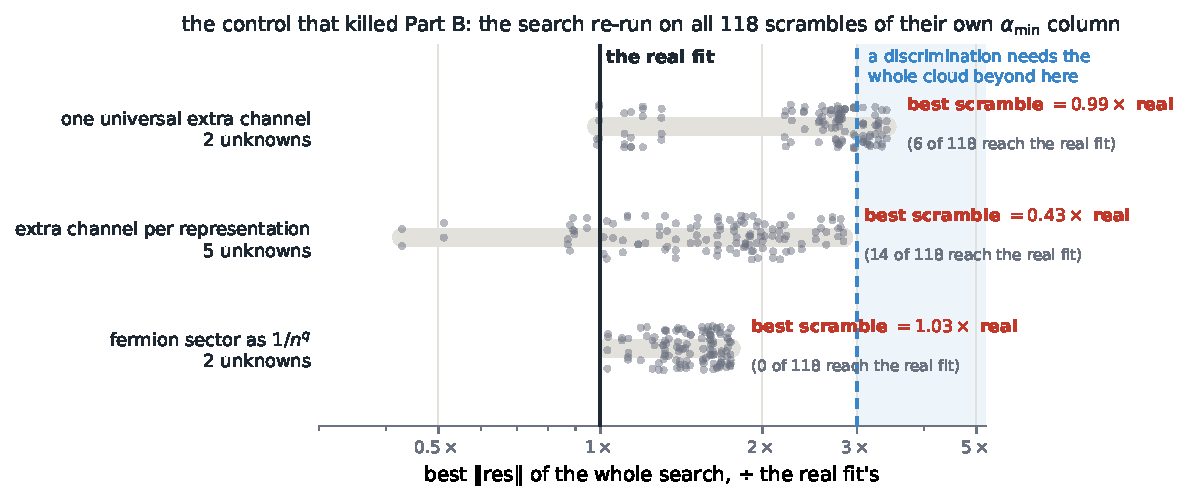
\includegraphics[width=\textwidth]{fig_anchor_controls.pdf}
\caption{The control that decides \S\ref{sec:instrument}'s last exclusion. Each candidate repair is
a scan --- one extra channel $v\sum_n s^n\cos(c\pi n\alpha)/n^p$ over $c\in[0.5,40]$,
$p\in\{3,\dots,7\}$, $s=\pm1$, or the fermion sector run as $1/n^q$ --- so the control must re-run
the \emph{whole scan} on scrambled data, not re-solve at the winning parameters. Grey dots: the best
residual of the full search on each of the $118$ non-trivial permutations of their own $\amin$
column, divided by the real fit's. A discrimination needs the whole cloud beyond the dashed
threshold; every cloud instead straddles $1$, and on two of the three tests the scrambled data
\emph{beats} the real data. Generated by \texttt{make\_figures\_su7.py}.}
\label{fig:controls}
\end{figure}

\textbf{And it is not one extra channel.} The three remaining candidates --- a cosine argument
outside $\{1,2,3\}\times\pi n\alpha$, an $n$-dependence that is not $1/n^5$, or multiplets not in
(69),(70) --- are one object, $\delta(\alpha)=v\sum_n s^n\cos(c\pi n\alpha)/n^p$, and the system
stays linear. Scanning $(c,p,s)$ and re-running the entire scan on all $118$ permutations of their
$\amin$ column (Fig.~\ref{fig:controls}) gives scramble bests of $0.99\times$ and $0.43\times$ the
real fit, and $51$ of the $80$ values of $c$ lie within $3\times$ of the winner: a forest, not a
minimum. The $1/n^q$ variant needs the fermion sector $15\times$ weaker than their own eq.~(72).

\textbf{And their own table is not a misprint.} Their eq.~(82) makes the third column of Table~1 a
function of the first, $1/R_5=2\times80.4~\text{GeV}/\amin$, and we had used the first two for three
days without checking it. All five rows are consistent: each printed pair $(\amin,1/R_5)$ has a
non-empty common interval at two significant figures. So the discrepancy is about the potential and
not about a number that was typed wrong --- a possibility that had never been closed. On rows (3)
and (4), the two that fail everything else, the $1/R_5$ column is in fact the \emph{sharper}
constraint on $\amin$, at $20\,\%$ and $35\,\%$ of the naive width; intersecting the boxes moves the
minimum residual only from $0.1561$ to $0.1563$, so it buys precision and no new exclusion.

\textbf{And the instrument is not generically broken.} Every exclusion above is internal to this
computation. The external question --- whether a one-loop Wilson-line potential assembled this way
reproduces a \emph{published} gauge-Higgs vacuum at all --- is answered in Part~V of this series,
against a 6D $\su4$ paper with an author in common \cite{AHMN}: the vacuum comes out exactly,
$(0.438,0.299)$ against $(0.438,0.299)$, and the Higgs mass ratio to $0.1\,\%$. That comparison was
made on ratios, so it was blind to the one thing an $\amin$ discrepancy could be --- an overall
mis-normalisation. It is not one: their three published mass-matrix elements meet ours through a
\emph{single} constant at a spread of $0.54\,\%$, and that constant is $1/4\pi^7$, the prefactor of
their own eq.~(4.1), which was no input of ours. Their $\lambda_{\min}$ then comes out $0.058799$
against their $0.058791$. That is a different implementation --- Part~V's is built from Schur
characters on two Wilson phases, this one counts components of one --- so it does not show the
$\su7$ assembly is right. It shows the approach reproduces a published 6D vacuum \emph{and its
absolute scale}, which removes global normalisation from the list of things the anchor failure could
be.

\begin{observation}[the exclusion list above is the one-loop list, and it is not the whole space]
\label{obs:looporder}
Everything excluded in this section lives at one loop, and the three structural candidates named
above are the one-loop candidates. There is a fourth: \emph{loop order}. The Wilson-line potential is
the Polyakov-loop potential of thermal gauge theory, where the two-loop calculation is old. At two
loops in pure gauge it is a multiplicative, background-independent rescaling of the one-loop result,
$\Omega^{(2)}/\Omega^{(1)}=-5g^2C_2(A)/(16\pi^2)$ for any classical or exceptional group
\cite{DGKA} --- which is excluded here already, because the $\lambda$ the $\amin$ column wants is not
one number. With fermions that proportionality fails \cite{GuoDu}, and the expressions carry
Bernoulli polynomials of the individual background angles \emph{and of their pairwise differences}.
Those angles are the Wilson-line charges, so a product of two such structures generates cosines at
$c_b\pm c_d$: with $c\in\{1,2,3\}$ that reaches $c\in\{0,\dots,6\}$, and $4,5,6$ lie outside the set.
Numerically $5g^2C_2(A)/(16\pi^2)$ is $7$--$14\,\%$ for $g_4\in[0.55,0.80]$ at $C_2(A)=7$, against
the $4$--$20\,\%$ rescaling the $\amin$ column asks for: \emph{the same order}. We have not computed
this term for this model and nothing here depends on it; what it establishes is that the list above
is the one-loop list. It does not rescue Table~1 either, since their potential, their $m_h$ and the
finiteness that motivates gauge-Higgs unification are all one-loop statements. The bounded question
it leaves is group-theoretic and needs no loop integral, and we answer it: \emph{does the two-loop
fermionic potential depend on the representation only through the multiset of its charges?} It does
not. With $\mathrm{Tr}(T^aT^b)=\delta^{ab}/2$, their weight is exactly $2\sum_a|T^a_{ij}|^2$ on the
fundamental, so the general-$R$ replacement is forced to be
$W(w,w')=\sum_a|\langle w|T^a_R|w'\rangle|^2$, whose row sums are $C_2(R)$; and
$\rep{48}^{(+)}$ against $4\times\rep7^{(+)}+\rep7^{(-)}+\rep{28}^{(+)}$ have identical one-loop
term tables --- hence identical $F$, $\amin$, $m_h$ and $D$ --- with $\sum C_2$ of $7$ against
$24.8571$. The one-loop potential is blind to the charge-zero states, so it fixes the Dynkin index
and not the Casimir. Neither member of that pair is a Table~1 content, so nothing published here is
separated by it.
\end{observation}

\begin{observation}[the guard lied first, and it is recorded]
The first version of that control was this programme's usual one: fix $(c,p,s)$ at the winner,
reverse the $\amin$ column, re-solve. It returns ratios $3.41$ and $3.51$ and the verdict
``informative'' on tests that are dead. Scanning is itself a search, so a control that does not
re-run the search measures nothing. Both the broken guard and the fix are in the archived output.
\end{observation}

One diagnostic is worth reporting because it is sharp and we cannot place it. At their published
$\alpha$, rows (1), (2) and (5) satisfy the $m_h$ invariant with our \emph{unmodified} $F''$ at
$g_4=0.60322$, $0.61847$ and $0.59943$, close to the Standard-Model $\su2_L$ value $0.63$; row (4) is off
by a
factor 3; and row (3) --- the row they single out and plot in their Fig.~2 --- has
$F''(0.021)=-2.44883317179876457187207506193<0$, exact, so their eq.~(80) returns no real Higgs mass
there at all. The potential does not turn convex until $\alpha=0.0238002801693$, which is
$1.133\times$ their $\amin$.
The exact value comes from a closed form worth recording on its own: every term of the potential is
$\mathrm{Re}\,\mathrm{Li}_5\!\left(s\,e^{ic\pi\alpha}\right)$, so
\[
F(\alpha)=\sum_{\text{terms}}m\,\mathrm{Re}\,\mathrm{Li}_5\!\left(s\,e^{ic\pi\alpha}\right),
\qquad
F''(\alpha)=-\sum_{\text{terms}}m\,(c\pi)^2\,\mathrm{Re}\,\mathrm{Li}_3\!\left(s\,e^{ic\pi\alpha}\right),
\]
with no truncation --- which matters, because $F''$ is the slowly converging $1/n^3$ series.

\paragraph{Where the residual sits, with the confound stated in the same breath.} The two rows that
fail are exactly the two whose content contains a $\rep{48}$ --- (3) with $3\times\rep{48}$, (4) with
$2\times\rep{48}$ --- and the one linear system the $\amin$ column \emph{does} satisfy asks for
$w(\rep{48})=5.59$, the largest single reweighting anywhere in this section. That number deserves the
error bar it has never carried, because the $\rep{48}$ is the badly conditioned coordinate here: it
is $99\,\%$ of the softest singular direction of the design matrix, at a singular value $75$ times
below the stiffest. It survives anyway. The residual profile has a genuine minimum there rather than
a plateau, and propagating the only noise these data have --- their two significant figures ---
gives $w(\rep{48})\in[5.20,6.00]$ at $95\,\%$, a relative width of $14\,\%$ against $1\,\%$ for
$w(\rep{84})$, still excluding $1$ by a factor of five. A soft direction is badly measured only
relative to the noise, and here the noise is two decimal places of a table. Two instruments that
share no arithmetic point at the same multiplet, which is to say at their eq.~(75). The confound
belongs beside it: those two rows are also exactly the two with the smallest $\amin$, and with five
rows the two readings cannot be separated. What would separate them is a sixth published row --- a
content with a $\rep{48}$ at large $\amin$, or one without at small --- and no such published truth
exists.

It could, though, and that is worth pinning down rather than leaving as a regret. Of the $427$
contents that break electroweak symmetry among the six fermions their own text allows, $22$ land in
$120$--$132$~GeV, a band around their own selection window; and within that band the two $\amin$
ranges \emph{overlap}, $[0.0180,0.0734]$ with a $\rep{48}$ against $[0.0288,0.0873]$ without. The
lock between the two readings is therefore an accident of the five rows they chose, not a property
of the model. The cleanest breaker is
$\rep{28}^{(+,-)}+\rep{28}^{(+,+)}+\rep{48}^{(+,+)}+3\times\rep{84}^{(+,+)}$, which we put at
$\amin=0.0734$ and $m_h=126.2$~GeV --- inside their own $125$--$127$ window, and carrying a
$\rep{48}$ at an $\amin$ larger than any $\rep{48}$ row they printed.

\begin{keyeq}
\textbf{So the prediction can be written before the row exists.} On their five rows
$\amin^{\rm ours}/\amin^{\rm theirs}$ is $1.94$ where there is a $\rep{48}$ and $1.20$ where there is
not. For that content the two readings therefore commit to different numbers: a published $\amin$
near $0.0378$ if the $\rep{48}$ is the locus, near $0.0612$ if small $\amin$ is. They differ by a
factor $1.62$, which two significant figures resolve. We adopt neither, and record both.
\end{keyeq}

\noindent
Against the $\rep{48}$ reading, their eq.~(75) is transcribed correctly twice over, by hand
from $s=\eta\eta'$ and by an independent state count on the $\su2$ generated by $T^{44}$, both giving
multiplicities $1,2,8$. So \emph{if} the $\rep{48}$ is the locus, what is wrong is not our reading of
their equation --- and that is a claim about someone else's paper which five data points do not
support and which we do not make. It is recorded because it turns ``we cannot reproduce Table~1''
into a question with an address.

\begin{keyeq}
This is stated as \textbf{a question for the authors and not as a defect claim}. Three independent
transcription controls pass, so a residual we cannot place is more likely ours than theirs;
\S\ref{sec:scope} states the scope that leaves. The
question has a location and a witness: \emph{which ingredient of \S3.2 takes eqs.~(68) and
(72)--(76) to the $\amin$ of Table~1?}
\end{keyeq}

\bridge{An open instrument is only fatal if the conclusion depends on it. How much of the instrument
does a verdict that is the sign of one rational number actually touch?}

% ===================================================================
\section{Why the discrepancy does not reach the conclusion}\label{sec:repair}

The honest objection to \S\ref{sec:vacuum} is that $D$ is computed from the very equations that fail
in \S\ref{sec:instrument}. We answer it not at a point but over a region: treat the residual as an
unknown per-representation reweighting $w_R$ --- the most general \emph{multiplicative} deformation,
and the family that contains every repair the data has ever asked for --- and ask for which $w$ the
conclusion survives.

$D$ is exactly linear in $w$, and the per-multiplet coefficients are the table of
\S\ref{sec:vacuum}. Two things follow immediately.

\begin{keyeq}
\textbf{(i) $D(\rep{48}^{(+,+)})=0$ identically in $w(\rep{48})$.} The $\rep{48}$ contributes
$mc^2=1\cdot4+2\cdot1=6$ at $s=+1$ and $8\cdot1=8$ at $s=-1$, and $6-\tfrac34\cdot8=0$. The monomial
is \emph{absent} from the polynomial, not small in it. So $w(\rep{48})=5.59$ --- the single largest
repair the $\amin$ column asks for, and the one linear system the anchor data \emph{does} satisfy
--- is invisible to the conclusion. Not approximately: identically.

\textbf{(ii) The conclusion is the wedge}
\[
2\,w(\rep{28})+\tfrac54\,w(\rep{84})\;<\;\tfrac{27}{8}\;<\;2\,w(\rep{28})+\tfrac{15}{4}\,w(\rep{84}),
\]
the left inequality being ``case (3) dies'' and the right ``case (2) lives''. Neither $w(\rep7)$ nor
$w(\rep{48})$ appears: the conclusion lives in a plane.
\end{keyeq}

\paragraph{The same zero does opposite duty in \S\ref{sec:ladder}, and it is worth saying so plainly.}
Here $D(\rep{48})=0$ is what makes the conclusion \emph{robust}: the worst-fitted weight in the paper
cannot touch it. There it is what makes the conclusion \emph{precarious}: a $\rep{48}$ donated for
free would cost case (3) nothing, and case (3) holds three. One number, two roles, no contradiction
--- the first is about reweighting a multiplet that stays in the potential, the second about removing
one from it.

\begin{figure}[t]
\centering
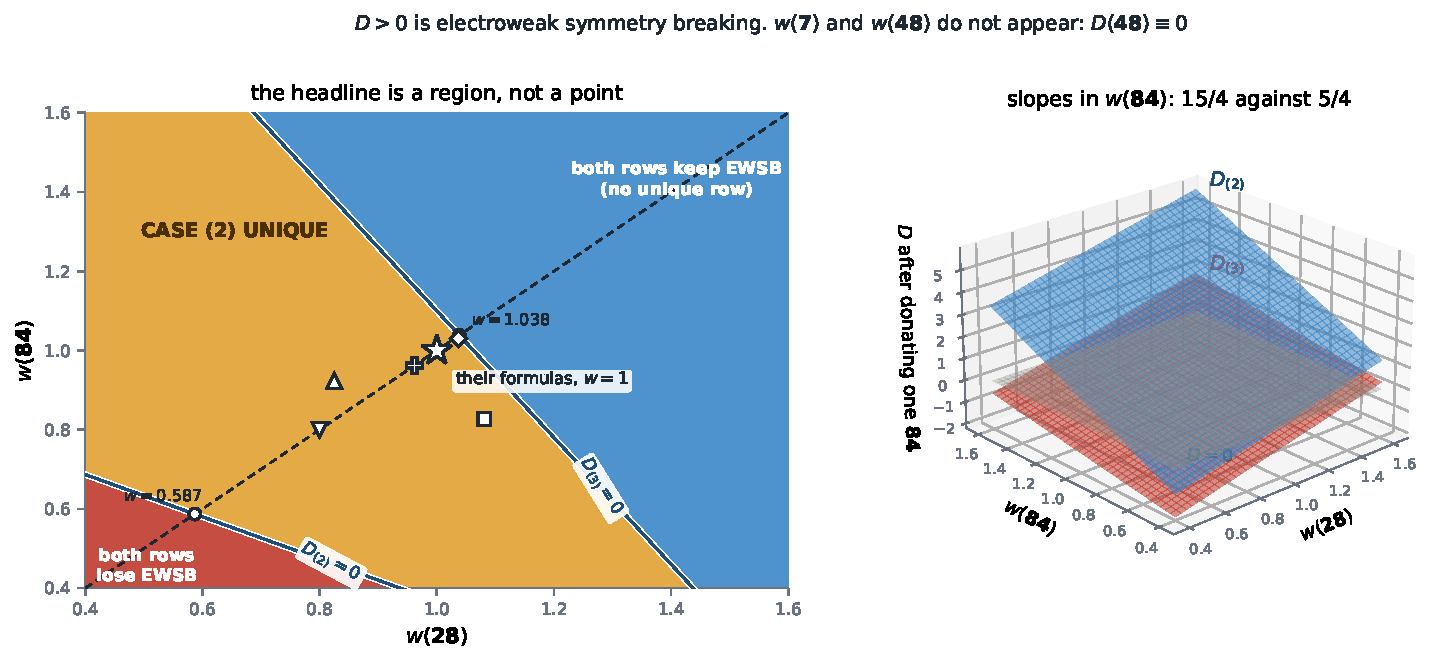
\includegraphics[width=\textwidth]{fig_repair_space.pdf}
\caption{\textbf{Left:} the $(w(\rep{28}),w(\rep{84}))$ plane, coloured by verdict after donating one
$\rep{84}^{(+,+)}$. The amber region is where case (2) survives and case (3) does not --- the
conclusion of this paper. Open marks are every repair the anchor discrepancy has ever been fitted to
(\S\ref{sec:instrument}); all of them lie inside it, and so does $w=1$. The dashed diagonal carries
the interval $(27/46,\,27/26)=(0.587,\,1.038)$, which reproduces the $\lambda_{\rm crit}$ of
\S\ref{sec:vacuum} by a different route. \textbf{Right:} why it is a wedge --- $D$ for the two rows
is two planes over the same square, with slopes $15/4$ and $5/4$ in $w(\rep{84})$, and the
conclusion is the slab between their zero sets. Generated by \texttt{make\_figures\_su7.py}.}
\label{fig:repair}
\end{figure}

Since $D_{(2)}-D_{(3)}=\tfrac52\,w(\rep{84})>0$ for any positive weight, row (3) can never outlive
row (2); the plane has three regions and not four. Sliced along $w(\rep{28})=w(\rep{84})=w$ the
boundaries are the exact rationals $27/46=0.5870$ and $27/26=1.0385$, which are precisely the
$\lambda_{\rm crit}$ of \S\ref{sec:vacuum} reached by an independent route. \textbf{The conclusion
holds on the whole interval $w\in(0.5870,1.0385)$, a factor $1.77$ wide, and that interval contains
$w=1$.} Every repair ever fitted lies inside the wedge (Fig.~\ref{fig:repair}); the thinnest margin
is the curvature-only system at $w(\rep{84})=1.030$ against a ceiling of $1.0385$, and that system is
exactly determined and therefore says nothing --- but it is where a sceptical reader should push,
and we say so rather than smoothing it.

The per-channel reweighting of \S\ref{sec:instrument} dies a third time here, on an instrument that
never sees $\amin$ or $m_h$: at the channel weights that fit ($0.13$--$0.28$, where their eq.~(72)
says $1$), all five rows have $D<0$ --- \emph{no electroweak symmetry breaking at all}, including
in the rows whose published numbers the fit was constructed to reproduce. A repair that reproduces
two numbers of a row by destroying the phenomenon the row exists to exhibit is not a repair.

Finally, the whole of \S\ref{sec:vacuum} was rebuilt from group theory alone, with their
eqs.~(73)--(76) never consulted: from the Wilson-line charge basis $u,v=(5\pm7)/\sqrt2$ and the
per-index parity $\pi=P_5P_5'=(+,+,+,-,-,+,-)$, the decompositions $\rep{28}=\mathrm{Sym}^2(\rep7)$,
$\rep{84}=\mathrm{Sym}^3(\rep7)$ and $\rep{48}=\rep7\otimes\rep{\bar7}-\rep1$ reproduce every term
multiplicity, every per-multiplet $D$, and both boundaries $27/46$ and $27/26$, symbolically in
$\mathbb{Q}[w_7,w_{28},w_{48},w_{84}]$. The $\rep{28}$ is built there as $\mathrm{Sym}^2(\rep7)$
and not as the conjugate identified in \S\ref{sec:setting}, and that is not an inconsistency:
conjugation reverses the sign of every charge and leaves every parity, while $D$ sees the charge
only through $c=2|q|$ with the states already paired as $\pm q$. The two readings give the same $D$
term by term. That construction never applies the $(1,\rep4)$ rule of
their eq.~(71) --- the quadruplet's smaller eigenvalue is simply a $\mathrm{Sym}^3(\rep7)$ component
at charge $1/2$, counted like any other --- and lands on the same $12$ regardless, which confirms
their one-sentence rule from the other side.

\paragraph{The wedge is a one-loop statement, and it is thinnest exactly where the open question is.}
The gauge coefficient $27/8$ is held fixed above, and at one loop that is right: the gauge part is
rebuilt and not fitted, and \S\ref{sec:setting} derives it from the adjoint's own charge-and-parity
table rather than from their eq.~(62) --- which matters here and nowhere else, since this is the one
weight the wedge does not let float. Only the \emph{ratio} of the fermion weight to the
gauge weight enters, and the wedge says it lies in $(27/46,\,27/26)$. The two margins from $1$ are
not symmetric: $19/46=41.304\,\%$ below, and $1/26=3.846\,\%$ above. Equivalently --- and this is the
form that matters --- suppressing the gauge sector alone by more than $1/27=3.7037\,\%$ makes row (3)
survive the donation as well, and case (2) stops being unique. A rescaling common to both sectors
changes nothing whatever, which is asserted rather than assumed.

That threshold should be read against Observation~\ref{obs:looporder}. The one candidate for the
missing ingredient this paper cannot exclude is loop order, and a two-loop term does not respect the
split: in pure gauge it multiplies the gauge sector by $1-5g^2C_2(A)/(16\pi^2)$, which at
$C_2(A)=7$ is $6.70$--$14.19\,\%$ over $g_4\in[0.55,0.80]$, while with fermions the proportionality
is known to fail \cite{GuoDu}. That is between $1.8$ and $3.8$ times the margin.

\paragraph{And that estimate is too crude, in the direction that matters.} It reads the alarm off
the \emph{gauge-only} suppression, but the fermion sector is suppressed as well, and by how much is
published in the same place: \cite{GuoDu}'s eq.~(5.13) gives
$\Gamma^{(2)}_f/\Gamma^{(1)}_f=-3g^2C_F(N)/(8\pi^2)$ against \cite{DGKA}'s
$-5g^2C_2(A)/(16\pi^2)$, so
\[
  \frac{\delta_f}{\delta_b}=\underbrace{\frac{6}{5}}_{\text{4D integrals}}\cdot
  \underbrace{\frac{C_F}{C_2(A)}}_{\text{group theory}}
  =\frac{3(N^2-1)}{5N^2}=\frac{144}{245}=0.5878 \quad\text{at } N=7 .
\]
The two factors must be kept apart, and the second is the only one that transfers: the $6/5$ is
$(3/8)\big/(5/16)$, a ratio of \emph{four-dimensional} loop coefficients. Group theory alone gives
$C_F/C_2(A)=(N^2-1)/2N^2<1/2$, so it takes a coefficient ratio above $2N^2/(N^2-1)\simeq2.04$ to
make the fermion sector the more suppressed one and send $w$ down; in four dimensions that ratio is
$1.2$. The conclusion that \textbf{$w$ rises} is therefore \emph{robust} --- it survives a factor
$1.7$ of error in the transplanted coefficients --- but it is not a theorem, and it is not stated as
one. Only the size depends on $g_4$. Correcting the estimate for the fermionic half, the gauge-only
equivalent of the net effect, $1/(1-s)=(1+\delta_f)/(1+\delta_b)$, is $2.88\,\%$ at $g_4=0.55$ and
$6.38\,\%$ at $g_4=0.80$: not $1.8$--$3.8$ times the margin but $0.78$--$1.72$, crossing it at
$g_4=0.6205$. At the $g_4=0.63$ this series uses it sits at $1.033$ times the margin ---
\emph{over the ceiling, by $0.13\,\%$}.

So the alarm is much smaller than the paragraph above states and much sharper: a knife edge at the
nominal coupling rather than a factor of four. It is stated here at its true size and on the wrong
side, because that is where it falls. What keeps it from being a verdict is that both inputs are
four-dimensional and thermal --- their group factors are this same algebra, their loop integrals are
not --- and that \cite{GuoDu}'s clean proportionality is their chemical-potential sector, their
background-dependent ratio (5.12) being no proportionality at all, as they say themselves. The
transplant is reported as a transplant. Its lesson is not that the conclusion fails but that the
open question cannot be assumed to fall the safe way: the closest published analogue falls the other
way, at the nominal coupling, by less than half a percent. Computed in
\texttt{twoloop\_wedge.py}, with the control that a rescaling common to both sectors returns exactly
$1$.

Stated there it reads as an alarm, and an earlier draft answered it with the anchor data: $\amin$ is
monotone increasing in the fermion weight on all five rows and ours is too \emph{large} on all five,
so the reweighting the $\amin$ column asks for is a \emph{suppression} of the fermion sector, and
solving $\arg\min F=\amin^{\rm theirs}$ row by row gives $0.8483$, $0.9619$, $0.8102$, $0.7996$,
$0.8480$ --- every one inside the wedge and every one \emph{below} $1$
(\texttt{su7\_\allowbreak wedge\_\allowbreak direction.py}, whose archived output still carries them).

\textbf{That answer is withdrawn, and the reason is worth more than the answer was.} Those five
numbers are a \emph{fit}, not a measurement of $w$. They say what uniform reweighting would
reproduce each row \emph{separately}, and a uniform reweighting would give one number: they give
five, spread over $20\,\%$ from $0.7996$ to $0.9619$. A residual that is not uniform is not a
reweighting, and the companion Part~VII localises it elsewhere --- its second published anchor
validates the potential and the minimiser, leaving the model-specific dictionary as what remains to
be explained. A mis-assigned parity or charge changes the potential term by term, which is exactly
how a fit to it scatters. So the five numbers measure the size of that discrepancy in weight units,
row by row, and carry no information about where the physical $w$ sits.

Removing the fit removes the defence. At one loop $w=1$ by construction, the gauge sector being
rebuilt and not fitted; and the estimate below puts the two-loop transplant at $1.0398$ against the
ceiling of $1.0385$. \textbf{Nothing in the anchor data pushes back on that, and the earlier draft
said it did.} What the anchor data does say is what \S\ref{sec:instrument} already claims of it: the
discrepancy is real, unexplained, and located in the dictionary rather than the machinery.

\begin{figure}[t]
\centering
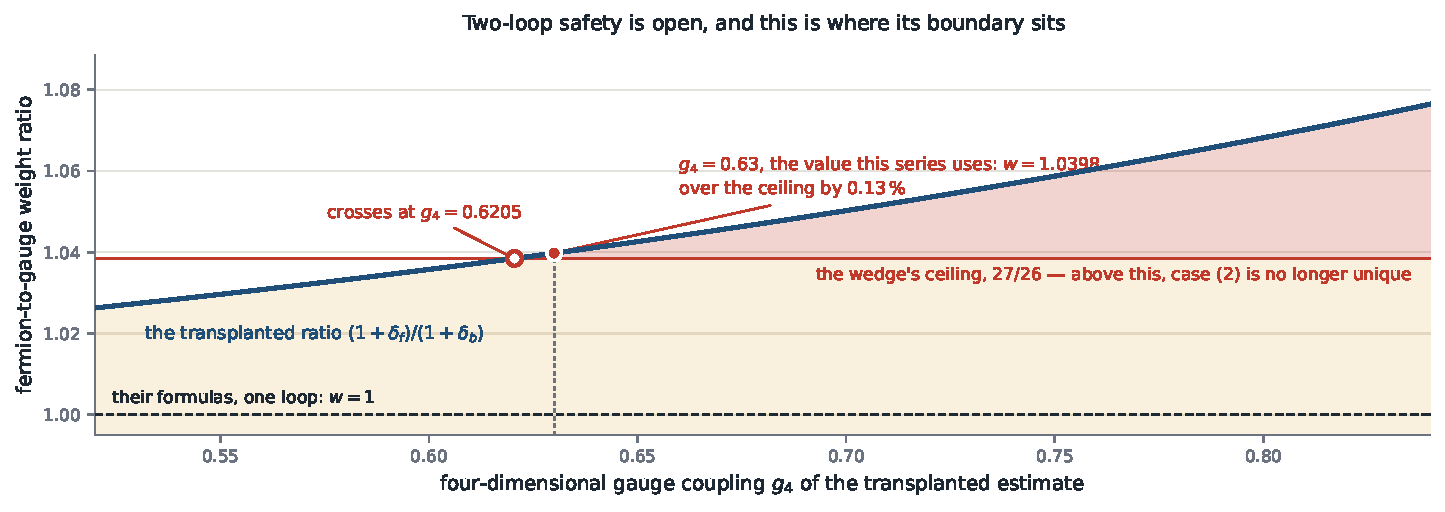
\includegraphics[width=\textwidth]{fig_ratio_line.pdf}
\caption{Where the boundary of validity of this paper's verdict sits. The verdict is a statement
about one number, the fermion-to-gauge weight ratio $w$; \S\ref{sec:repair} shows it holds on the
wedge, whose ceiling is $27/26$ (red). What the wedge does not absorb is loop order, so the curve is
the transplanted two-loop ratio $(1+\delta_f)/(1+\delta_b)$ built from \cite{DGKA}'s gauge half and
\cite{GuoDu}'s fermionic one, against the four-dimensional coupling of those results. It crosses the
ceiling at $g_4=0.6205$, and at the $g_4=0.63$ this series uses it sits $0.13\,\%$ above: on the
\emph{wrong} side, and by less than half a per cent. \textbf{Not drawn, and deliberately: the five
row-by-row reweightings the $\amin$ column asks for.} They are a fit and not a measurement of $w$,
the argument that used them is withdrawn on the previous page, and a figure may not keep making an
argument the text has retracted. Drawn by \texttt{make\_figures\_su7.py} from the archived
\texttt{twoloop\_wedge.json}.}
\label{fig:ratio}
\end{figure}

\begin{keyeq}
\textbf{Two-loop safety is open, and this is where the boundary of validity sits.} The verdict is
robust over the whole family of multiplicative one-loop deformations: the wedge $(27/46,\,27/26)$
contains $w=1$ and every repair the discrepancy has ever been fitted to. \textbf{A two-loop term
need not belong to that family} --- it is under no obligation to be a uniform rescaling of anything
(\S\ref{sec:open}), so there may be no effective $w$ for it to move. The closest published analogue,
four-dimensional and thermal in both halves, puts the transplanted ratio at $1.0398$ against the
ceiling $1.0385$: on the dangerous side, at the nominal coupling, by less than half a per cent, and
it crosses at $g_4=0.6205$ (Fig.~\ref{fig:ratio}). That
transplant does not settle the six-dimensional question and nothing here claims it does. What it
does is locate the boundary exactly.
\end{keyeq}

\noindent
So the exposure is stated at its true size and on the side it actually falls, rather than argued
away. This paper had an argument that it fell the safe way, and that argument is the one withdrawn
above: it read a direction off five row-by-row fits, and five fits that scatter by $20\,\%$ measure
the discrepancy rather than the weight. What would settle the question is the six-dimensional
calculation nobody has done. Its bounded group-theoretic half needs no loop integral and is answered
here --- Observation~\ref{obs:looporder}, and the first two entries of \S\ref{sec:open}: two loops
does see content one loop cannot, so the ratio cannot be assumed to be $1$.

\bridge{Every step above borrowed a mechanism from somebody. The last job of the argument is to say
from whom, and where the borrowing stops.}

% ===================================================================
\section{Attribution}\label{sec:scope}

\textbf{Every mechanism used here is someone else's}, and the following gates were run before the
corresponding results were written, not after.

% a longtable, not a tabular: as an unbreakable box this ran to nearly a page and
% could not fit under its own section heading, stranding it with 312pt of white
\begingroup\small
\begin{longtable}{p{0.55\textwidth}p{0.38\textwidth}}
\toprule
\rowcolor{hdrblue!12}
mechanism & status\\
\midrule
\endfirsthead
\toprule
\rowcolor{hdrblue!12}
mechanism & status\\
\midrule
\endhead
the anomaly-free $U(1)$ extensions of the Standard Model are
$\mathrm{span}\{Y,B-L\}$, and gauged $B-L$ needs right-handed neutrinos of charge $-1$ &
textbook, forty years old\\
a gauged $B-L$ fails to forbid the $B-L$-conserving proton operators; the cure is a
family-dependent $B-x_iL$ & \cite{FamilyU1}, verbatim in its abstract; the dimension-6 statement is
Weinberg and Wilczek--Zee \cite{Weinberg,WZ}\\
placing families in different representations or at different fixed points of an orbifold GUT, and
thereby suppressing proton decay & standard orbifold-GUT model building \cite{Raby,OrbGUT}\\
a broken extra $U(1)$ leaves a residual \emph{discrete gauge} symmetry that can forbid the
dimension-4, -5 and -6 proton operators & \cite{KW,IR,DiscGauge,Orth}\\
localised anomalies constrain brane charges, and Green--Schwarz can absorb mixed $U(1)$ ones &
von Gersdorff--Quir\'os; Kojima--Takenaga--Yamashita \cite{KTY}, which \cite{KM25} cite as their
ref.~[13]\\
brane fields in orbifold GUTs need not furnish representations inherited from the bulk & standard
practice; it is why their own quarks can be localised at all\\
matter in the adjoint --- a real representation --- is vector-like, and it is a $\ZZ_3$ projection
that chiralises it & \cite{GMN}, verbatim in its introduction: \emph{``It is well known that\dots\
The matter in the adjoint representation is always vector-like, but one can project out the
vector-like partner by a $Z_3$ transformation.''} Proposition~\ref{prop:real} is the specialisation
to their $\pm1$ diagonal parities, where that cure is unavailable; the counts and the chiral controls
are ours\\
a leftover $U(1)$ in gauge-Higgs unification broken by a scalar with a vacuum expectation value of
order $1/R$, with the surviving charge read off the direction of that value & \cite{GHK},
eqs.~(50)--(54), (77), (79) --- the mechanism of \S\ref{sec:qphi} is theirs\\
no local brane Yukawa for the charged leptons in gauge-Higgs unification, and the obstruction is
called generic & \cite{SSS,Maru19} --- relevant to the rung-by-rung Yukawa closure of
\S\ref{sec:ladder}, which is why that closure is a control and not a result\\
\rowcolor{amber!13}
a rule of thumb selecting the fermion content from the curvature of the Wilson-line potential
\emph{at the origin} & \cite{AdachiMaru}. This is the closest prior art to \S\ref{sec:vacuum}: their
Hessian factorises at $\alpha=0$ and their selection rule is our arithmetic --- \textbf{at the
origin, and only there}. What is not theirs is the exact rational $D$ per multiplet, and the
donation cost that follows from it\\
minimality plus anomaly cancellation fixing the Standard-Model family content &
\cite{GengMarshak} --- background to \S\ref{sec:anom}, which is a relative statement inside a fixed
model rather than a classification\\
\bottomrule
\end{longtable}
\endgroup

\textbf{What is ours} is the specialisation to their model: that their own eqs.~(43)--(47) and
(76)--(79) force $U(1)'=T_{3L}+Y-(B-L)$ and therefore no protection at one generation; that their
spectrum requires a right-handed neutrino of charge $-1$ that only the $\rep{28}$ supplies --- and
that it is required rather than merely sufficient --- and that only rows (2) and (3) contain it; the
rung ladder inside their $\su7$, the identity of Proposition~\ref{prop:identity}, the fourteen
surviving assignments together with the two of them their own tensors can host, and that the
$\rep{84}^{(+,+)}$ hosting rung 1 is already in every row of their Table~1; the closed form
$V''(0)=-\pi^2\zeta(3)D$ with its rational per-multiplet table, and the selection of case (2) as the
only published row that survives both conditions; the closed-form selection rule $q_\varphi=|A_j|/n$
with its maximum, and
$q_\varphi=3/2$ as a universal protector by a mod-3 argument; the invariant $K$ of
\S\ref{sec:instrument}; and the region result of \S\ref{sec:repair}.

\textbf{What is not claimed.}
\emph{Any $\amin$, $1/R_5$ or $m_h$ for any modified content} --- the instrument of
\S\ref{sec:instrument} forbids it, and everything above is stated as a sign, an exact rational or a
closed form precisely for that reason. \emph{That case (2) works}: what is shown is that it is the
only candidate left; making it work is their computation as much as ours. \textbf{That leaves a
question we can state precisely and cannot answer here: after the donation, does the surviving
row still land in $m_h=125$--$127$~GeV?} Answering it needs the modified potential minimised, which needs a closed form for $\amin$ this paper does not have; Part~VII \cite{PartVII} supplies one and answers it.
\emph{Any vacuum expectation value, scale, coefficient or lifetime} --- \S\ref{sec:qphi} is a
selection rule, not a prediction of $\tau_p$. \emph{Operators above dimension 6}, whose charges were
not enumerated. \emph{That more than one scalar does not break $U(1)'$} --- with several the
residual group is fixed by $\gcd(q_1,q_2,\dots)$, which can only make protection harder.
\emph{That the mixed $U(1)$ anomalies must cancel on localised matter} --- Green--Schwarz remains
available, and turning it on makes the result of \S\ref{sec:qphi} stronger rather than weaker, which
is the unusual direction. \emph{That the anchor discrepancy is theirs} --- three controls pass, so
a residual we cannot place is more likely ours. \emph{And no defect in their paper anywhere in this
work}: what \S\ref{sec:instrument} reports is an open question, and what \S\ref{sec:setting} reports
about the $\rep{28}$ and about $\pi_5=\pi_7$ are unstated data with computed consequences.

Their paper has \emph{one} generation --- the words \emph{generation} and \emph{family} do not occur
in it outside a reference title --- so \S\ref{sec:ladder} onwards is about the three-generation
extension their model must eventually have and does not yet have. Getting three generations is
itself an unstated problem in their paper; the escape lives exactly inside it.

\bridge{That is what the paper does, and whose each mechanism is. Before asking what it leaves
open, it is worth putting every claim it does make on one page, with the control that stands
behind each --- including the two controls that came back saying \emph{untested}.}

% ===================================================================
\section{Verification}\label{sec:verif}

Every claim above is collected here once, against the evidence that carries it. Where a
statement is proved the entry is the proof and the control on its implementation; where it is
only measured, the entry says so, and where a control could have fired and did not the entry
says that too. \textbf{A claim whose control also passes on scrambled data is recorded as
untested, not as confirmed} --- two of them are, and they are the two worth reading twice.
The last two blocks are the ones a referee should start from: what is \emph{open}, and what an
earlier draft claimed and this one retracts.

\begingroup
\small
\begin{longtable}{p{0.62\textwidth}p{0.31\textwidth}}
\caption{Every claim of this paper against the evidence that carries it. The blocks are, in order:
what is claimed; what is reported as \emph{data} of \cite{KM25} rather than as a defect; what is
\emph{open}; and what an earlier draft claimed and this one retracts.}\\
\toprule
\rowcolor{hdrblue!12}
\textbf{Claim} & \textbf{Where, and on what}\\
\midrule
\endfirsthead
\toprule
\rowcolor{hdrblue!12}
\textbf{Claim} & \textbf{Where, and on what}\\
\midrule
\endhead
Three anomaly channels force $X_Q=-1/6$, which is exactly $A=0$ & \S\ref{sec:anom}; six channels,
re-derived independently under Sage from the $A_6$ character ring\\
$U(1)'=T_{3L}+Y-(B-L)$ on every field, and all four operators have $Y=B-L=0$ & \S\ref{sec:anom},
an identity\\
Two channels cannot cancel and demand a singlet of charge $-1$; it exists in the $\rep{28}$ and
nowhere else, so only rows (2),(3) supply it & \S\ref{sec:anom}; $\sum x=-1$ and $\sum x^3=-1$ are
independent\\
A $\rep{28}$ is \emph{necessary} and not merely minimal: the solution set is $e=-1-4w$, $u=5w$, so
the net $\rep{28}$ number is never zero & \S\ref{sec:anom}; and a brute-force scan with no $\rep{28}$
returns nothing while the same scan with one condition dropped returns solutions\\
Only two of the fourteen assignments fit inside their own tensors, and both require charge $-1$ &
\S\ref{sec:ladder}; rung $\ge2$ is unhostable --- four boxes for the tensor powers, and for the
$\rep{48}$, which is not one, no chiral zero mode. The fourteen are re-derived by an
independent implementation\\
\rowcolor{amber!12}Proposition~\ref{prop:real} --- the mechanism is \cite{GMN}'s, the specialisation
ours: under their $\pm1$ diagonal parities a real representation furnishes no chiral generation, so
the $\rep{48}$ cannot host the escape --- and a $\rep{48}^{(+,+)}$ would have cost
$D=0$ exactly & \S\ref{sec:ladder}, proved in three lines and counted in
\texttt{su7\_adjoint\_is\_vectorlike.py}, with the $\rep{28}$ and
$\rep{84}$ as the control that must come out chiral and does ($10$ and $34$ unpaired states). Case
(3) holds three $\rep{48}$s, so this is a step and not an aside\\
Their eq.~(81), quoted for the 5D $\su4$ model, is forced by their own eq.~(54): the $W$ carries
Wilson-line charge $\tfrac12$ and the photon $0$ & \S\ref{sec:setting}; the charge-$1$ modes exist,
so the control is not vacuous\\
$\mathrm{extra}(L)=(1-k)/2$, and $\mathrm{extra}(L)+\mathrm{extra}(e^c)=1/2$ on every rung &
\S\ref{sec:ladder}; rung 0 returns their own eq.~(43)\\
Proposition~\ref{prop:identity}: $[\su2_L]^2U(1)'=\tfrac12\sum_jA_j$ & \S\ref{sec:ladder}, exact;
14 assignments survive all six channels\\
Rung 1 is hosted by an $\rep{84}^{(+,+)}$, which is in every row of Table~1; the $\rep{35}$ cannot
host it & \S\ref{sec:ladder}, from their eqs.~(37)--(40)\\
$V''(0)=-\pi^2\zeta(3)D$, $D$ rational; $\rep{48}^{(+,+)}\mapsto0$, $\rep{84}^{(+,+)}\mapsto5/4$ &
\S\ref{sec:vacuum}; the truncation residual is \emph{predicted} to $2\,\%$\\
\rowcolor{amber!12}\textbf{Case (2) is the only one of the five published rows that supplies the
$\nu_R$ and survives the donation --- within the minimal extension, at one-loop curvature} &
\S\ref{sec:anom} $+$ \S\ref{sec:vacuum}, Fig.~\ref{fig:verdicts}; everything in eighths. A benchmark
selected, not a model delivered: the modified potential is not recomputed. \emph{Depends on their
eq.~(67)}: the verdict holds on $w\in[74/99,118/151)$ and only $w=3/4$ is admissible there\\
Proposition~\ref{prop:closed}: protection fails iff $q_\varphi=|A_j|/n$; the set has a maximum &
\S\ref{sec:qphi}; $18\,648$ brute-scan values, $0$ disagreements\\
$q_\varphi=3/2$ forbids all four operators to all orders for every half-integer $X_Q$ &
\S\ref{sec:qphi}; and $q_\varphi=1/2$, $1$ both fail, so it is not vacuous\\
$K=m_h\amin/\sqrt{F''(\amin)}$ is row-independent, $R_5,R_6,k$ cancelling & \S\ref{sec:instrument},
verified symbolically\\
$D(\rep{48})\equiv0$, and the conclusion is a wedge containing $w=1$ and every fitted repair &
\S\ref{sec:repair}, Fig.~\ref{fig:repair}; rebuilt from group theory in Sage\\
Their $\rep{48}$-subscripted terms in eq.~(76) must be $\rep{84}$ terms, identified by a count &
\S\ref{sec:instrument}; the $\rep{84}$'s fifteen doublets come out only then\\
$F=\sum m\,\mathrm{Re}\,\mathrm{Li}_5(s\,e^{ic\pi\alpha})$ and $F''$ a sum of
$\mathrm{Re}\,\mathrm{Li}_3$, with no truncation & \S\ref{sec:instrument}, verified in Sage; it is
what makes the $30$-digit $F''(0.021)$ exact\\
Their eqs.~(54),(41),(57),(69),(70) and their KK spectrum are derived, not assumed, and nothing in
them is wrong & \S\ref{sec:setting}; $13/13$ structure constants, the omitted one exactly zero,
charges $\{0,\pm\tfrac12,\pm1\}$ with multiplicities $26,20,2$\\
Their eq.~(68) too: its three coefficients follow from the adjoint's
$(q,P_5P_5',P_6)$ table with two weights, $a=2$ and $b=\tfrac12$ &
\S\ref{sec:setting}; overdetermined, and the two rows that fix $a$ agree. This is the sector the
wedge holds fixed, and it was the only one checked against nothing but their own eq.~(62)\\
\midrule
\rowcolor{hdrblue!10}\textbf{Unstated in their paper, reported as data and not as defects} &
\textbf{Where}\\
\midrule
Their $\rep{28}$ is $\mathrm{Sym}^2(\rep{\bar7})$, the conjugate & \S\ref{sec:setting}; $4/4$ against
$2/4$, and the test discriminates ($\rep{84}$: $10/10$ against $1/10$). Invisible to $V_{\rm eff}$\\
$\pi_5=\pi_7$: the two indices the Wilson line mixes carry the same $P_5P_5'$, without which their
eq.~(72) is not well defined & \S\ref{sec:setting}, \S\ref{sec:repair}; the first thing the Sage
construction checks\\
Their spectrum requires a right-handed neutrino, not stated in their paper &
\S\ref{sec:anom}\\
Their Table~1 is internally consistent: eq.~(82) makes $1/R_5$ a function of $\amin$, and all five
printed pairs agree & \S\ref{sec:instrument}; a control on \emph{their} table that could have fired.
On rows (3),(4) the $1/R_5$ column is the sharper constraint\\
\midrule
\rowcolor{hdrblue!10}\textbf{Open, and stated as open} & \textbf{Why}\\
\midrule
Their Table~1 $\amin$ is not reproduced from their eqs.~(68),(72)--(76) & \S\ref{sec:instrument};
gauge sector exact, truncation irrelevant, transcription verified three ways, no multiplicative or
single-channel repair survives its control\\
Case (3) has $F''<0$ at its own published $\amin$ under our assembly & \S\ref{sec:instrument}; exact
to 30 digits, and the inflection is at $1.133\times$ that value\\
\rowcolor{hdrblue!7}\textbf{The exclusion list above is the \emph{one-loop} list} &
\S\ref{sec:instrument}, Observation~\ref{obs:looporder}. Two-loop pure gauge is multiplicative and
therefore already excluded; with fermions it is not, and its size is the same order as the
rescaling the $\amin$ column wants. Not computed here, and stated so\\
\rowcolor{warmred!12}\textbf{And so is the wedge}: it tolerates $1/27$ of relative
gauge-versus-fermion rescaling, and the published two-loop rescalings put the transplant
\emph{over} it at the nominal coupling &
\S\ref{sec:repair}. With \cite{GuoDu}'s fermionic half included, $0.78$--$1.72$ times the margin
over $g_4\in[0.55,0.80]$ --- not the $1.8$--$3.8$ of a gauge-only reading --- crossing at
$g_4=0.6205$ and at $1.033$ at $g_4=0.63$. An earlier draft answered this with the anchor column;
that answer is \textbf{withdrawn}\\
\rowcolor{warmred!12}\textbf{And both inputs of that estimate are four-dimensional and thermal} &
their group factors are this algebra, their loop integrals are not, and the $6/5$ is made of the
latter. \cite{DGKA} add a limitation of their own, in their own words: they have \emph{``not
succeeded in finding a general proof''} of eq.~(66) that avoids explicit evaluation, and do not know
how the combinatorics works \emph{inside} the Weyl chamber --- their proof covers the straight paths
from the origin to the $Z(N)$ minima, along its edges. An $\amin\simeq0.05$ is on neither\\
The two rows that fail are exactly the two containing a $\rep{48}$, and the one satisfiable system
asks for $w(\rep{48})=5.59$, $[5.20,6.00]$ at $95\,\%$ under their own rounding &
\S\ref{sec:instrument}; confounded with their being the two smallest $\amin$, and five rows cannot
separate the readings. Their eq.~(75) is verified twice over, so no defect is claimed\\
The instrument is validated only \emph{as an approach} & \S\ref{sec:instrument}: Part~V's
independent implementation reproduces \cite{AHMN} exactly, but it is a different implementation, so
it does not certify the $\su7$ assembly\\
\midrule
\rowcolor{warmred!14}\textbf{Retracted, and left visible} & \textbf{Why}\\
\midrule
``the exact eqs.~(62)--(65) need $k\approx1.2$'' & never computed; a conclusion line printed as a
literal string. The real correction is $1.5\,\%$ at $k=1.2$. \S\ref{sec:instrument}\\
``one extra channel repairs the anchor, and the control says it is informative'' & the control fixed
the winner instead of re-running the search. \S\ref{sec:instrument}, Fig.~\ref{fig:controls}\\
\bottomrule
\end{longtable}
\endgroup

\bridge{Read down that ledger and the open items are the rows with neither a proof nor a
measurement. What does each of them need, and which of them can this paper's own instrument
already make precise enough to hand to somebody?}

% ===================================================================
\section{Open problems}\label{sec:open}

\S\ref{sec:verif} recorded what is carried. This is the other list: what the work \emph{opens}.
Each entry names the quantity that decides it, the threshold that quantity must cross, and the test
that would settle it --- a question with no discriminating test is a mood rather than a problem ---
and each says which line of work it belongs to, because in every case the lineage is what makes the
question precise rather than merely unanswered. They are in the order in which one hands the next
its data.

\paragraph{1. Does the two-loop fermionic term raise the fermion-to-gauge ratio, or lower it?}
That one sign decides \S\ref{sec:repair}: raising it past $27/26$ costs the verdict, lowering it
costs nothing and would explain the anchor. It is now two margins and not one, and they are
independent: the wedge of \S\ref{sec:repair} measures how far the \emph{weight of a multiplet} may
move, and the window $w\in[74/99,118/151)$ of \S\ref{sec:vacuum} measures how far the
\emph{alternating ratio} may move. A two-loop term need respect neither --- it is not obliged to be a
uniform rescaling of anything --- so both margins are quoted, and a calculation that lands outside
either one changes the answer. The group-theoretic half is already done, and it answers
already: the two-loop matter factor is \emph{not} determined by the one-loop charge multiset. The
weight replacing \cite{GuoDu}'s on a general representation is forced to be
$W(w,w')=\sum_a|\langle w|T^a_R|w'\rangle|^2$, whose row sums are $C_2(R)$, and it is \emph{not} a
function of the multiset of charges --- so a two-loop term sees content that one loop cannot, and the
ratio cannot be assumed to be $1$. What is missing is the loop integrals in six dimensions, where the
Bernoulli structure of the four-dimensional thermal calculation has never been carried. That gap is
not ours to name: the two-loop Wilson-line potential of gauge-Higgs unification has been computed
once, by \cite{HMTY} --- \cite{AdachiMaru}'s author among them --- for QED on $M^4\times S^1$, and
their own introduction says why it stopped there: \emph{``Evaluation of the Higgs mass at the two loop
level is formidable in non-Abelian gauge theory. To get insight in the problem it is instructive to
examine, as the first step, QED on $M^4\times S^1$.''} Nineteen years on, the non-Abelian
general-representation case is still that first step's sequel. The
observable that separates the two loop orders exists and is exhibited: $\rep{48}^{(+)}$ against
$4\times\rep7^{(+)}+\rep7^{(-)}+\rep{28}^{(+)}$ have identical one-loop term tables --- hence
identical $F$, $\amin$, $m_h$ and $D$ --- and $\sum C_2$ of $7$ against $24.8571$. \emph{Ours, and
the hardest thing here.}

\paragraph{1b. And how far that ``sees more'' goes, which is bounded --- and the bound needs no loop
integral either.} The answer above is a negative with no ceiling on it: two loops sees content one
loop cannot, and nothing said how much more. What can be said, and by counting rather than computing,
is what \emph{kind} of representation data a second loop is allowed to use:

\begin{quote}
\textbf{at two loops no matter trace of order higher than quadratic can occur}, so what the second
loop adds is \emph{charge-resolved quadratic data} and not a higher Casimir invariant.
\end{quote}

\noindent
That is a statement about the order of the trace, not a classification of two-loop topologies, and
the difference matters below.

Write the matter-dependent group factor of a two-loop vacuum diagram as a trace over the
representation. The sunset factor $\sum_a\mathrm{tr}_R(T^a f(H) T^a g(H))$ reduces, root class by
root class, to five tables of a \emph{single} charge, because for a root with
$\Delta=\langle\alpha,T\rangle$ fixed the second charge is determined:
\[
  N_\Delta(q)\;=\!\!\sum_{w:\,q_w=q}\ \sum_{\alpha:\,\langle\alpha,T\rangle=\Delta}
  \bigl|\langle w+\alpha|E^\alpha|w\rangle\bigr|^2 ,
\]
and two contents give the same sunset \emph{whatever the loop integrals are} exactly when their five
tables agree --- the integrals are a common factor and cancel in the comparison. Their sum needs no
matrix element at all: from $C_2=\sum_i H_i^2+\sum_\alpha E^\alpha E^{-\alpha}$,
$\sum_\Delta N_\Delta(q)=\sum_{w:q_w=q}\mathrm{mult}(w)[C_2(R)-|w|^2]$. Computed on the witness by
$su(2)_\alpha$ string decomposition, all five tables agree at all eleven charges, on both contents,
with the Casimir identity reproducing the string result at $11$ of $11$ as an independent check.

That leaves the ingredient \cite{HMTY} name as their own frontier --- \emph{``there appear a new
interaction vertex proportional to $H$''} --- and it is settled by counting rather than computing.
For a connected vacuum graph $2I=\sum_k kV_k$, so
\[
  L \;=\; I-V+1 \;=\; 1+\tfrac12\sum_k V_k\,(k-2),
\]
the loop number depending on the \emph{valences} alone. A background leg is an external classical
field: $k$ counts the \emph{quantum} legs entering a vertex once the background has been inserted,
so a background leg carries no internal half-edge and cannot change $I$ or $V$, though it does
change the vertex tensor. Hence an insertion on a matter line and a three-gluon vertex
carrying a background leg are both weight zero: they may be added without limit and change nothing.
Writing $a$ for matter-gauge cubic vertices and $b$ for seagulls, the order of the matter trace on a
loop is $a+2b$, and at two loops $a+2b\le a+2b+c+2d+g=2$. \textbf{A cubic trace requires $a+2b\ge3$,
hence weight $\ge3$, hence $L\ge3$: no two-loop diagram can carry one.} Figure~\ref{fig:twoloop}.
The background cannot supply the missing adjoint index either, being a fixed Cartan direction.

So the two statements are complements and not rivals. Two loops does see content one loop cannot ---
that is the pair above, and it is why the ratio cannot be assumed. But what it sees is still
quadratic in the quantum generators, resolved by the background charges: the tables $N_\Delta(q)$,
and no invariant of higher order.

\textbf{What this is not, said before a referee has to ask.} The valence count bounds the
\emph{order} of the matter trace on a loop. It is not an enumeration of two-loop topologies, and the
following are not classified here: diagrams carrying more than one matter loop, the distinct
contractions of adjoint indices among them, six-dimensional counterterms and localised
contributions, and the non-abelian vertex structures beyond the one \cite{HMTY} name. Two contents
agreeing on the five tables therefore agree on the sunset factor and on every two-loop group factor
built from a single matter trace --- which is what the count reaches --- rather than on the two-loop
potential entire. Within that scope the conclusion is the useful one: \emph{a degeneracy that
survives $C_2$ is not waiting for a higher Casimir to lift it.}

What the count does not supply is the number that entry~1 turns on. It bounds the \emph{kind} of
representation data a second loop may use; the sign of $\delta_f/\delta_b-1$ still needs the
six-dimensional integrals. Nor can the published data supply it: five rows and one free ratio, with
the two rows that fail sharing both a $\rep{48}$ and the two smallest $\amin$. That degeneracy in
the data is the next entry.

\begin{figure}[t]
\centering
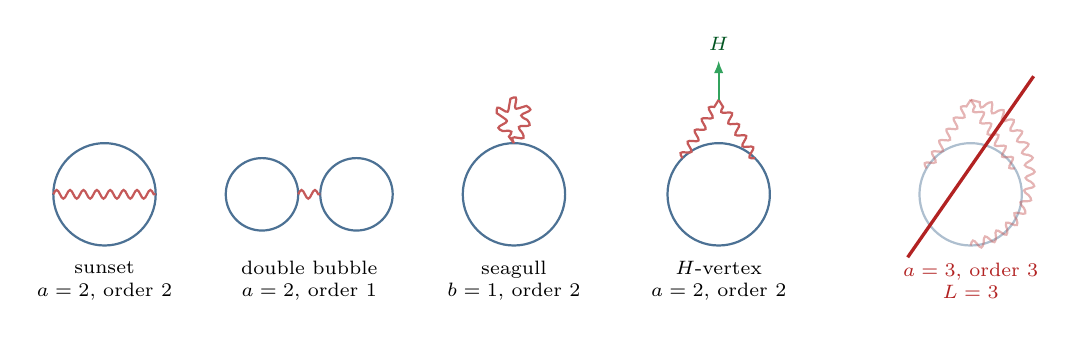
\begin{tikzpicture}[
  every node/.style={font=\scriptsize},
  matter/.style={draw=hdrblue!80,thick},
  gauge/.style={draw=warmred!75,thick,decorate,
                decoration={coil,aspect=0,segment length=1.7mm,amplitude=0.55mm}},
  bg/.style={-{Latex[length=1.6mm]},okgreen!80,thick},
  lbl/.style={font=\scriptsize,align=center}]

\def\R{6.5mm}
\foreach \x/\name/\ord in {0/sunset/2, 30/double bubble/1, 60/seagull/2, 90/$H$-vertex/2}{}

% --- 1. sunset
\begin{scope}[xshift=0mm]
  \draw[matter] (0,0) circle (\R);
  \draw[gauge] (-\R,0) -- (\R,0);
  \node[lbl] at (0,-11mm) {sunset\\ $a=2$,\ order $2$};
\end{scope}
% --- 2. double bubble
\begin{scope}[xshift=26mm]
  \draw[matter] (-6mm,0) circle (4.6mm);
  \draw[matter] (6mm,0) circle (4.6mm);
  \draw[gauge] (-1.4mm,0) -- (1.4mm,0);
  \node[lbl] at (0,-11mm) {double bubble\\ $a=2$,\ order $1$};
\end{scope}
% --- 3. seagull
\begin{scope}[xshift=52mm]
  \draw[matter] (0,0) circle (\R);
  \draw[gauge] (0,\R) .. controls (5mm,13mm) and (-5mm,13mm) .. (0,\R);
  \node[lbl] at (0,-11mm) {seagull\\ $b=1$,\ order $2$};
\end{scope}
% --- 4. H-vertex
\begin{scope}[xshift=78mm]
  \draw[matter] (0,0) circle (\R);
  \coordinate (v) at (0,12mm);
  \draw[gauge] (-4.6mm,4.6mm) -- (v);
  \draw[gauge] (4.6mm,4.6mm) -- (v);
  \draw[bg] (v) -- ++(0,5mm) node[above,okgreen!60!black] {$H$};
  \node[lbl] at (0,-11mm) {$H$-vertex\\ $a=2$,\ order $2$};
\end{scope}
% --- 5. excluded
\begin{scope}[xshift=110mm]
  \draw[matter,opacity=0.45] (0,0) circle (\R);
  \coordinate (u) at (0,12mm);
  \draw[gauge,opacity=0.45] (-5.6mm,3.3mm) -- (u);
  \draw[gauge,opacity=0.45] (5.6mm,3.3mm) -- (u);
  \draw[gauge,opacity=0.45] (0,-\R) .. controls (11mm,-4mm) and (9mm,10mm) .. (u);
  \draw[warmred,very thick] (-8mm,-8mm) -- (8mm,15mm);
  \node[lbl] at (0,-11mm) {\textcolor{warmred}{$a=3$,\ order $3$}\\\textcolor{warmred}{$L=3$}};
\end{scope}
\end{tikzpicture}
\caption{\textbf{Why the two-loop group factor cannot be cubic.} The loop number of a connected
vacuum graph is $L=1+\frac12\sum_k V_k(k-2)$, a function of the valences alone. Background legs
(green) are external classical fields and carry weight zero, so they may be attached without limit
--- including at the three-gluon vertex that \cite{HMTY} name as the non-abelian frontier, fourth
panel, which is a genuine two-loop diagram whose matter trace is nevertheless only
$\mathrm{tr}_R(T^aT^b)$: its new structure lives in the gauge vertex, hence in the integral, not in
the group factor. Only matter-gauge vertices carry both weight and a generator, so the trace order
$a+2b$ is bounded by the total weight $2$. The fifth panel is the cheapest way to a cubic trace and
it costs a third loop.}\label{fig:twoloop}
\end{figure}

\paragraph{2. A sixth row.} \S\ref{sec:instrument} pre-registers it: the content
$\rep{28}^{(+,-)}+\rep{28}^{(+,+)}+\rep{48}^{(+,+)}+3\times\rep{84}^{(+,+)}$ sits inside their own
$m_h$ window and carries a $\rep{48}$ at an $\amin$ larger than any $\rep{48}$ row they printed, and
the two readings of the residual commit to $0.0378$ against $0.0612$ for it, a factor $1.62$ apart
and therefore separated by two significant figures. \emph{Theirs, and it costs one minimisation.}

Such a row would also carry a second, independent obligation, and it is one nobody has to compute a
potential to check: whatever $\amin$ and $m_h$ it comes out with must return the same $K$ of
\eqref{eq:K} as every other row of the same table. That obligation is not particular to \cite{KM25},
which is the next entry.

\paragraph{3. How many published gauge-Higgs tables satisfy their own invariant?} $K$ of
\eqref{eq:K} is free to evaluate, needs no absolute normalisation, and must return one number on
every row of any table of this kind. We have run it on one paper, where it holds on three rows of
five, and anchored its absolute scale against a second, where three published mass-matrix elements
meet ours through a single constant. Neither is a survey. \emph{Ours.}

A survey would decide whether $K$ is a property of this class of models or an accident of two
papers. What it cannot reach is the row this one selects, which has no published $\amin$ to test
against at all.

\paragraph{4. Does case (2) work?} What is shown here is that it is the only candidate left, not
that it succeeds: whether a surviving row still lands at $m_h=125$--$127$~GeV once the
$\rep{84}^{(+,+)}$ is removed and three generations are in place is a computation this paper does not
do. \textbf{It is out of this paper's scope rather than open}: Part~VII \cite{PartVII} has the closed
form for $\amin$ that the computation needs and answers it, and the answer is that none of their five
rows lands in the window after the donation, with case~(2) the lowest of the four that still break.
What stays genuinely open is the rest of the model around that row --- the modified potential
minimised with the scalar sector of entry~5 in place --- and that potential cannot be written
before that sector is, which is the last entry. \emph{Theirs as much as ours.}

\paragraph{5. There is no complete effective action yet.} Two of the results above sit on a
branch that a localised-anomaly analysis would decide. Without Green--Schwarz, the brane charges are
tightly constrained and the permissive reading is forced by their own $X_Q=-1/6$; with it, $X_Q$ is
freed to $m/2$, a different space of assignments opens, and the $q_\varphi=3/2$ protection of
\S\ref{sec:qphi} becomes \emph{more} general rather than less. Both branches are stated here and
neither is closed, because closing them needs what nobody has written down for this model: the
effective action with every localised term and its cancellation mechanism made explicit --- and, with
it, the scalar sector that says why $U(1)'$ breaks in one direction and not another. That last part
is no longer an open-ended wish: \S\ref{sec:qphi} now says what such a sector has to \emph{do}. It
must leave the group generated by the $\rep{84}$ singlet --- on the strict half-integer lattice that
is $\ZZ_3$; on the permissive brane-charge branch the residual must be named only after the global
charge normalisation is fixed, the divisibility rule being the part that does not depend on it
(\S\ref{sec:qphi}) --- and, since the three charges their content supplies are
$\tfrac12,1,\tfrac32$ and all three pairs have $\gcd=\tfrac12$, it must give a vacuum expectation
value to the $\rep{84}$'s singlet and to \emph{neither} of the other two. That is a condition on a
potential, and a potential either meets it or does not. \emph{Theirs, and it is a construction
question rather than a computation.}

\medskip
\noindent
The six are one question asked at four depths. Part~V's negative result is that a one-loop
Wilson-line potential is blind to the charge-zero states, so it fixes the Dynkin index and not the
Casimir; that is why $D(\rep{48})=6-\tfrac34\cdot8=0$ identically, and entries 1 and 1b ask whether
a second loop restores the difference --- on the pair exhibited there, $\sum C_2$ of $7$ against
$24.8571$ at identical one-loop term tables. Entries 2 and 3 ask the same of the published data, one
table at a time. Entries 4 and 5 ask it of the model. The fourth is answered in Part~VII
\cite{PartVII}, which supplies the closed form for $\amin$ this paper does not have; the other five
are open at the time of writing.

% ===================================================================
\section*{Data availability}

\begingroup\raggedright\sloppy\emergencystretch=4em
Every displayed number in this paper regenerates from the ancillary scripts and is literally
greppable in the archived standard output beside them; a verifier enforces this and has fired twice.
A second one re-runs every script named below and diffs it against that archive, because the first
believes the archive: it caught two of these scripts having stopped running at all, their archived
numbers unchanged.
An interactive instrument for this series runs at
\href{https://karlesmarin.github.io/ghu-explorer/}{\texttt{karlesmarin.github.io/ghu-explorer}},
with source at \href{https://github.com/karlesmarin/ghu-explorer}{\texttt{github.com/karlesmarin/ghu-explorer}}. Its \emph{Anomalies \& proton} panel is this paper's
\S\ref{sec:vacuum} made usable: it prices every multiplet's contribution to $8D$ as signed bars,
draws the ladder of odd eighths with $8D=0$ marked as the rung that does not exist, and runs the
donation on each of their five rows, reporting what it costs and whether the row can pay ---
together with the same question asked of the whole lattice rather than of five rows. Every
number is computed in the reader's browser from the term tables, nothing is precomputed, and
each value carries a label saying whether it is a theorem, a verified check or a measurement
that inherits the anchor caveat of \S\ref{sec:instrument}.
The principal artifacts are \texttt{su7\_\allowbreak anomaly\_\allowbreak channels.py} and its independent Sage
re-derivation (\S\ref{sec:anom}), \texttt{su7\_\allowbreak family\_\allowbreak u1.py} (\S\ref{sec:ladder}),
\texttt{su7\_\allowbreak vacuum.py} (\S\ref{sec:vacuum}), \texttt{su7\_\allowbreak qphi.py} with the adversarial audit
\texttt{su7\_\allowbreak qphi\_\allowbreak socratic.py} (\S\ref{sec:qphi}), \texttt{su7\_\allowbreak anchor\_\allowbreak mh.py},
\texttt{su7\_\allowbreak anchor\_\allowbreak exact.sage}, \texttt{su7\_\allowbreak content\_\allowbreak dependence.py},
\texttt{su7\_\allowbreak kk\_\allowbreak spectrum.py} and \texttt{su7\_\allowbreak branchings.py} (\S\ref{sec:instrument}), and
\texttt{su7\_\allowbreak repair\_\allowbreak space.py} with \texttt{su7\_\allowbreak repair\_\allowbreak space.\allowbreak sage} (\S\ref{sec:repair}), and
\texttt{su7\_\allowbreak cross\_\allowbreak paper.py} for the three external checks of \S\ref{sec:instrument}.
\texttt{su7\_\allowbreak realisable.py} re-derives the fourteen assignments by an independent path and
carries the two that fit their content through \S\ref{sec:vacuum};
\texttt{su7\_\allowbreak w\_\allowbreak charge.py} is the $W$ Wilson-line charge of \S\ref{sec:setting}; and
\texttt{su7\_\allowbreak loop\_\allowbreak order\_\allowbreak margin.py} with \texttt{su7\_\allowbreak wedge\_\allowbreak direction.py} is the wedge
tolerance of \S\ref{sec:repair} and the side of it the data sits on;
\texttt{su7\_\allowbreak w48\_\allowbreak conditioning.py} is the error bar on $w(\rep{48})$; and
\texttt{su7\_\allowbreak gauge\_\allowbreak from\_\allowbreak group.py} rebuilds their eq.~(68) from the adjoint's
charge-and-parity table (\S\ref{sec:setting}), and
\texttt{su7\_\allowbreak fermion\_\allowbreak from\_\allowbreak group.py} does the same for their
eqs.~(73)--(76): all twenty blocks from the single rule $c=2|q|$, sign $=\eta\eta'P_5P_5'$, with the
$(1,\rep4)$ term switched off as the control that must fail --- and it folds their own
$\su2_L$ decomposition lists back onto the same numbers, which is the version of that count
that does not use $\dim=c+1$;
\texttt{su7\_\allowbreak residual\_\allowbreak group.py} names the residual group of
\S\ref{sec:qphi} and tabulates what a second condensing scalar does to it;
\texttt{su7\_\allowbreak adjoint\_\allowbreak is\_\allowbreak vectorlike.py} is the $\rep{48}$
exclusion of \S\ref{sec:ladder}, with \texttt{su7\_\allowbreak brane\_\allowbreak partner.py} the
adversarial run that made it necessary --- it prices the brane escape and finds every other gate
open; and
\texttt{su7\_\allowbreak D\_\allowbreak exponent.py} is the $w$-window of \S\ref{sec:vacuum}; and \texttt{su7\_\allowbreak sixth\_\allowbreak row.py}
is the pre-registered prediction of \S\ref{sec:instrument}. Figures~\ref{fig:verdicts}--\ref{fig:ratio}
are drawn by \texttt{make\_\allowbreak figures\_\allowbreak su7.py} from archived JSON, not recomputed;
Figures~\ref{fig:chain} and \ref{fig:twoloop} are drawn in this source.
\par\endgroup
\fussy

% ===================================================================
\section*{Acknowledgements}

This paper exists because of \cite{KM25}. Y.~Komori and N.~Maru wrote their model out fully enough
that a reader can rebuild its section~3 from its own equations, which is what \S\ref{sec:setting}
does --- and everything of theirs we checked came out right. They also said plainly what they had not
done, naming proton decay as future work. Stating an open question in public is a generous thing to
do, and everything from \S\ref{sec:anom} onwards is an attempt to pick it up rather than to mark it.
The one column we cannot reproduce is a question of ours, not a finding about them: three
transcription controls pass, and where the residual really sits we do not know.

N.~Maru replied promptly to a first set of questions about the construction, for which we are
grateful. He has not reviewed this paper: the reading of their equations here, and any error in it,
is entirely ours.

Almost nothing here is a new mechanism, and the ones we use cost other people a great deal of time.
Gogoladze, Mimura and Nandi \cite{GMN} state the vector-like character of adjoint matter and the
$\ZZ_3$ cure that escapes it; without their sentence, Proposition~\ref{prop:real} would have been
presented as a discovery instead of as a specialisation. Lee and Ma \cite{FamilyU1} supply the
family-dependent charge that \S\ref{sec:ladder} looks for inside $\su7$. Costa, Dobrescu and Fox
\cite{CDF} solved the gravitational and cubic $U(1)$ conditions in general, which is why \S\ref{sec:anom}
can say the $\rep{28}$ is \emph{necessary} rather than merely minimal. Adachi and Maru \cite{AdachiMaru}
had already read the curvature at the origin as a selection rule --- the closest prior art to
\S\ref{sec:vacuum}, and their rule of thumb is our arithmetic. Dumitru, Guo and Korthals Altes
\cite{DGKA} and Guo and Du \cite{GuoDu} computed the two-loop halves that \S\ref{sec:repair} borrows,
and were explicit about their own limits, which is what let us report the transplant as a transplant.
Hosotani, Maru, Takenaga and Yamashita \cite{HMTY} did the only two-loop Wilson-line potential in this
framework and wrote down why they stopped where they did; \S\ref{sec:open} quotes them because they
had already named the frontier. \S\ref{sec:scope} says which piece is whose, one by one, and that
table is the part of this paper we would most like a reader to check.

% ===================================================================
% Titles are given only where they are verified in our own archived reading of the source;
% elsewhere the identifier alone is cited. Nothing here is reconstructed from memory.
\begin{thebibliography}{99}\small
\setlength{\itemsep}{0pt plus 1pt}
\bibitem{KM25} Y.~Komori, N.~Maru, \emph{$SU(7)$ Grand Gauge-Higgs Unification}, NITEP 240,
arXiv:2503.04090.
\bibitem{AHMN} K.~Akamatsu, T.~Hirose, N.~Maru, A.~Nago, \emph{Electroweak Symmetry Breaking in Two
Higgs Doublet Model from 6D Gauge-Higgs Unification on $T^2/\ZZ_2$}, arXiv:2312.08608.
\bibitem{Manton} N.~S.~Manton, \emph{A new six-dimensional approach to the Weinberg--Salam model},
Nucl.\ Phys.\ \textbf{B158} (1979) 141.
\bibitem{Hosotani} Y.~Hosotani, Phys.\ Lett.\ \textbf{B126} (1983) 309; Ann.\ Phys.\ (N.Y.)
\textbf{190} (1989) 233.
\bibitem{Weinberg} S.~Weinberg, Phys.\ Rev.\ Lett.\ \textbf{43} (1979) 1566.
\bibitem{WZ} F.~Wilczek, A.~Zee, Phys.\ Rev.\ Lett.\ \textbf{43} (1979) 1571.
\bibitem{FamilyU1} H.-S.~Lee, E.~Ma, \emph{Gauged $B-x_iL$ origin of $R$ parity and its
implications}, arXiv:1001.0768. The family-dependent cure for a $B-L$ that cannot forbid the
$B-L$-conserving proton operators is stated verbatim in its abstract.
\bibitem{KW} L.~M.~Krauss, F.~Wilczek, \emph{Discrete gauge symmetry in continuum theories}, Phys.\
Rev.\ Lett.\ \textbf{62} (1989) 1221.
\bibitem{IR} L.~E.~Ib\'a\~nez, G.~G.~Ross, Nucl.\ Phys.\ \textbf{B368} (1992) 3.
\bibitem{DiscGauge} H.-S.~Lee, C.~Luhn, K.~T.~Matchev, \emph{Discrete gauge symmetries and proton
stability in the $U(1)'$-extended
MSSM}, JHEP \textbf{07} (2008) 065.
\bibitem{Orth} A.~Aranda, C.~D.~Carone, \emph{Orthogonal $U(1)$'s, proton stability and extra
dimensions}, hep-ph/0012092.
\bibitem{KTY} K.~Kojima, K.~Takenaga, T.~Yamashita, arXiv:1704.04840 --- cited by \cite{KM25} as
their ref.~[13].
\bibitem{GMN} I.~Gogoladze, Y.~Mimura, S.~Nandi, \emph{Model building with gauge-Yukawa
unification}, Phys.\ Rev.\ \textbf{D69} (2004) 075006, hep-ph/0311127 --- where the adjoint's
vector-like character is stated as well known and the $Z_3$ cure is named.
\bibitem{Raby} S.~Raby, \emph{Grand Unified Theories}, hep-ph/0608183 --- cited as a review of the
field; the orbifold constructions this paper actually leans on are \cite{OrbGUT}.
\bibitem{OrbGUT} A.~Kobakhidze, \emph{Proton stability in 5D GUTs with orbifold compactification},
hep-ph/0108049; A.~Hebecker, J.~March-Russell, \emph{Proton decay signatures of orbifold GUTs},
hep-ph/0204037.
\bibitem{SSS} C.~A.~Scrucca, M.~Serone, L.~Silvestrini, hep-ph/0304220 --- \cite{AHMN}'s own
ref.~[19].
\bibitem{Maru19} N.~Maru, arXiv:1903.08359 --- where the charged-lepton Yukawa obstruction is
called generic in gauge-Higgs unification.
\bibitem{AdachiMaru} T.~Adachi, N.~Maru, Phys.\ Rev.\ \textbf{D98} (2018) 015022,
arXiv:1804.06012.
\bibitem{GHK} P.~V.~Dong, \emph{A possible minimal gauge-Higgs unification}, arXiv:1105.0541,
eqs.~(50)--(54), (77), (79).
\bibitem{GengMarshak} C.~Q.~Geng, R.~E.~Marshak, Phys.\ Rev.\ \textbf{D39} (1989) 693.
\bibitem{CDF} D.~B.~Costa, B.~A.~Dobrescu, P.~J.~Fox, \emph{General Solution to the $U(1)$ Anomaly
Equations}, Phys.\ Rev.\ Lett.\ \textbf{123} (2019) 151601, arXiv:1905.13729 --- the gravitational
and cubic conditions as a Diophantine system, solved in general.
\bibitem{DGKA} A.~Dumitru, Y.~Guo, C.~P.~Korthals Altes, Phys.\ Rev.\ \textbf{D89} (2014) 016009,
arXiv:1305.6846, eq.~(66); and Bhattacharya, Gocksch, Korthals Altes, Pisarski, Nucl.\ Phys.\
\textbf{B383} (1992) 497.
\bibitem{GuoDu} Y.~Guo, Q.~Du, JHEP \textbf{05} (2019) 042, arXiv:1810.13090.
\bibitem{HMTY} Y.~Hosotani, N.~Maru, K.~Takenaga, T.~Yamashita, \emph{Two loop finiteness of Higgs
mass and potential in the gauge-Higgs unification}, Prog.\ Theor.\ Phys.\ \textbf{118} (2007) 1053,
arXiv:0709.2844 --- the only two-loop Wilson-line potential in this framework, and Abelian.
\bibitem{PartI} C.~Mar\'in, \emph{Anomaly- and Tadpole-Compatible Fermion Completion of
Six-Dimensional $\su4$ Gauge--Higgs Unification}, Part~I, doi:10.5281/zenodo.21432625.
\bibitem{PartII} C.~Mar\'in, \emph{Three Gates to a Quark Generation: an exact criterion for which
$\su4$ representations contain the Standard Model}, Part~II, doi:10.5281/zenodo.21432627.
\bibitem{PartIII} C.~Mar\'in, \emph{A Centre-Charge Selection Rule for the Wilson-Line Potential},
Part~III, doi:10.5281/zenodo.21438226.
\bibitem{PartIV} C.~Mar\'in, \emph{Schur Functions at $(1,-1,t,t^{-1})$: a closed form on the
non-identity component of $O(4)$}, Part~IV, doi:10.5281/zenodo.21463000.
\bibitem{PartVII} C.~Mar\'in, \emph{The compactification scale of $SU(7)$ grand gauge-Higgs
unification is bounded}, Part~VII of this series, to appear.
\bibitem{PartV} C.~Mar\'in, \emph{What the Higgs Potential Cannot See: bulk matter that cannot help
select a boundary condition}, Part~V, doi:10.5281/zenodo.21727094.
\end{thebibliography}
\end{document}
